\documentclass[letterpaper,12pt,oneside]{article}
\usepackage{amsmath}
\usepackage{amsfonts}
\usepackage{listings}
\usepackage{amssymb}
\usepackage{graphicx}
\usepackage[utf8]{inputenc}
\usepackage[left=2cm,right=2cm,top=2cm,bottom=2cm]{geometry}
\usepackage[spanish]{babel}    %caracteres en espa�ol
\usepackage{blindtext}% es para generar el texto de ejemplo
\usepackage{amsmath,amssymb,amsfonts}  %caracteres matem�ticos
\usepackage{hyperref} %referencias a ecuaciones con hiperv�nculos
\usepackage{fancyhdr} %encabezados y pies de p�gina
\usepackage{multicol,multirow} %unir celdas en tablas
\usepackage{parskip} %quita la sangr�a (comentar si quieres empezar los parrafos con sangria)
\usepackage{geometry} %margenes y esquemas
%EDITAR T�TULO AQU�!!!!!!!!!
\author{Profesor: Rina Ortiz\\
Nombre: Omar Herrera}
\title{An\'alisis de movimiento y morfolog\'ia de c\'elulas cancer\'igenas}
\begin{document}
\maketitle
En este documento se analizar\'an videos de movimiento de c\'elulas cancer\'igenas, para as\'i poder contribuir al avance de futuros estudios sobre el c\'ancer. Para esto se mostrar\'an gr\'aficos de \'area, largo y alto vs tiempo, as\'i como tambi\'en se mostrar\'an gr\'aficos de variaciones del \'area, largo y alto a medida que pasa el tiempo, luego se mostrar\'an correlaciones entre las distintas dimensiones de las c\'elulas y tambi\'en correlaciones entre las distintas dimensiones y la velocidad. Adem\'as se analiza la correlaci\'on entre el cociente del largo y alto con la velocidad, esto es para ver si es que a medida que las c\'elulas son m\'as compactas (o esf\'ericas) su velocidad aumenta o disminuye, adem\'as se hace un an\'alisis sobre la correlaci\'on entre la distancia recorrida por las c\'elulas y su \'area y finalmente se muestran los \'angulos de las c\'elulas considerando su posici\'on final e inicial.\\
A continuaci\'on se presentan los gr\'aficos de \'Area vs tiempo.\\
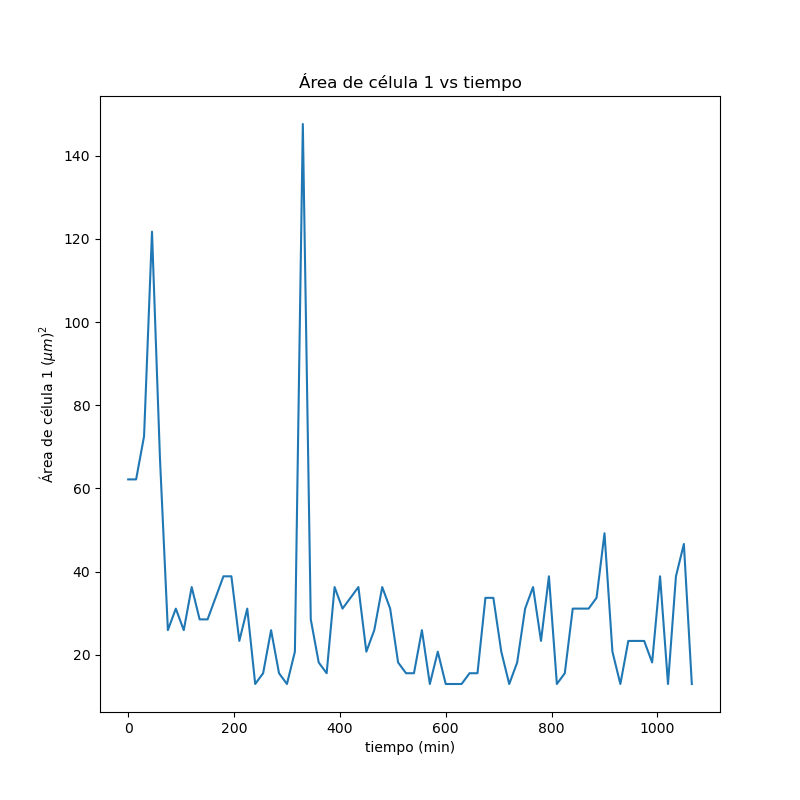
\includegraphics[scale=0.4]{Area_de_celula_1_vs_tiempo.png} 
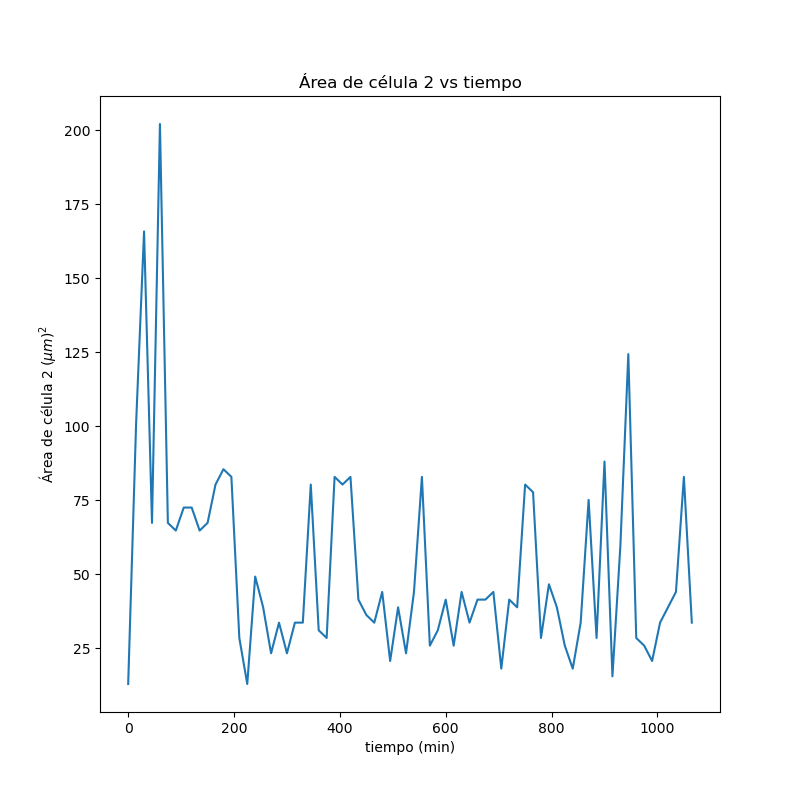
\includegraphics[scale=0.4]{Area_de_celula_2_vs_tiempo.png} 
\\
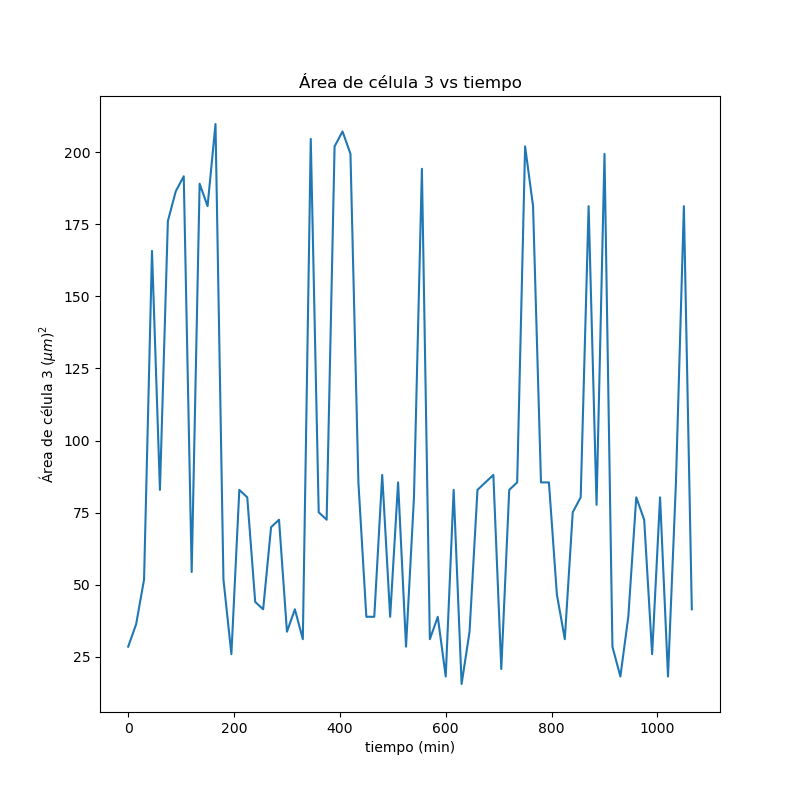
\includegraphics[scale=0.4]{Area_de_celula_3_vs_tiempo.png} 
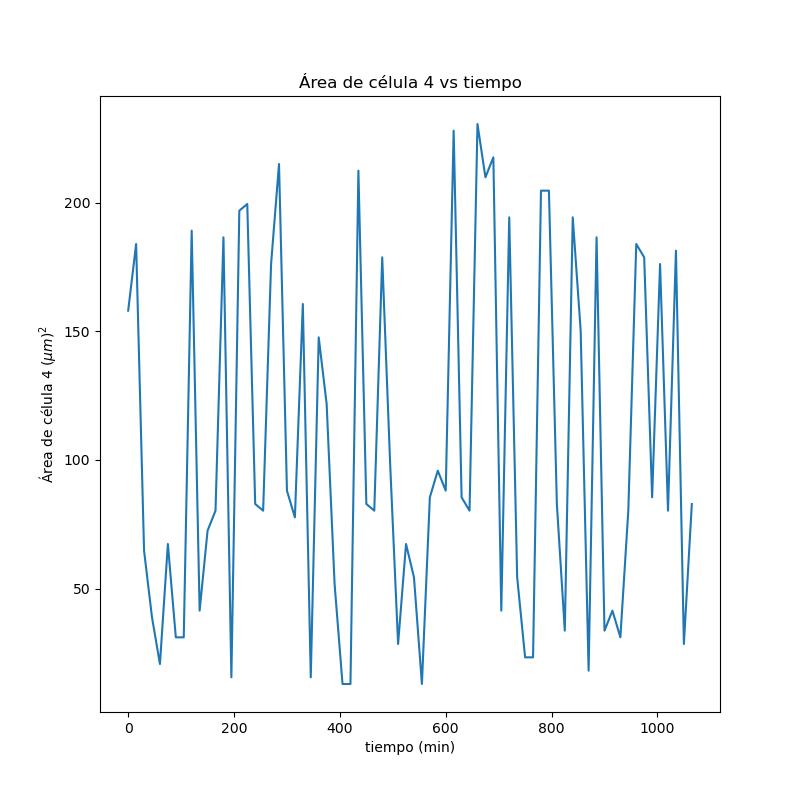
\includegraphics[scale=0.4]{Area_de_celula_4_vs_tiempo.png} 
\\
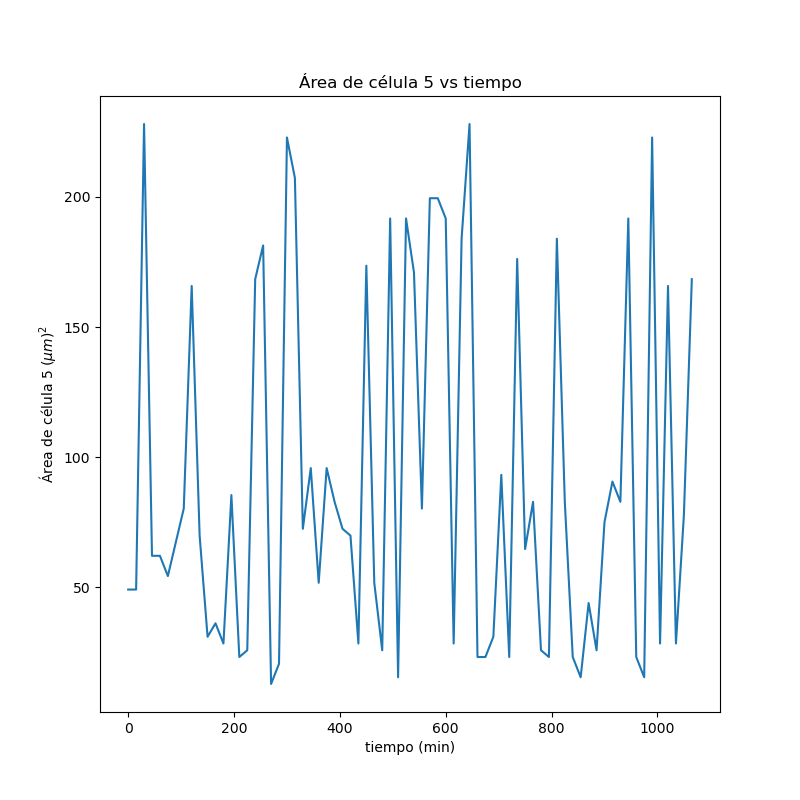
\includegraphics[scale=0.4]{Area_de_celula_5_vs_tiempo.png} 
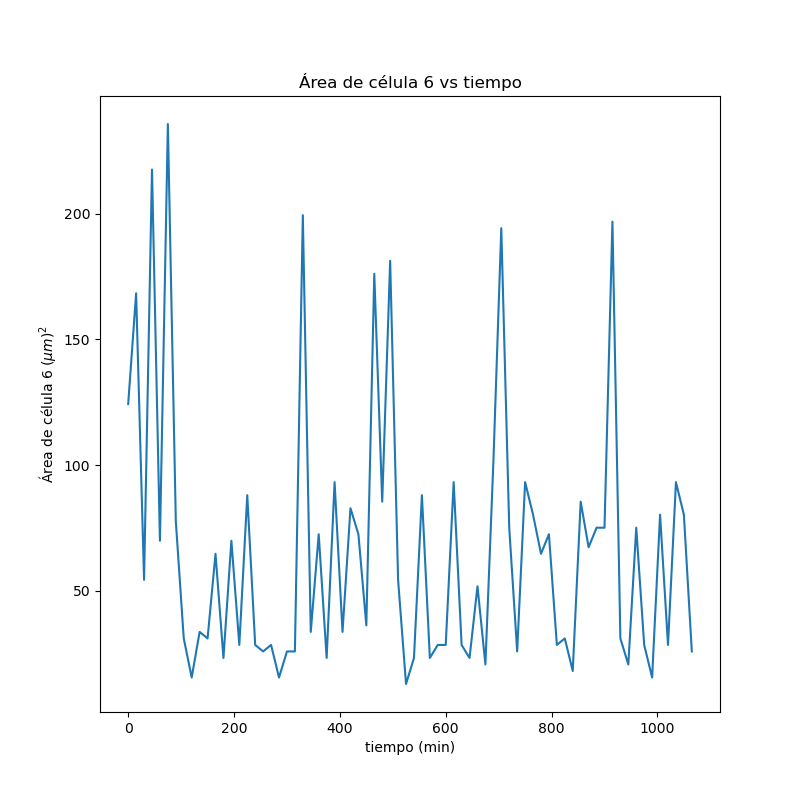
\includegraphics[scale=0.4]{Area_de_celula_6_vs_tiempo.png} 
\\
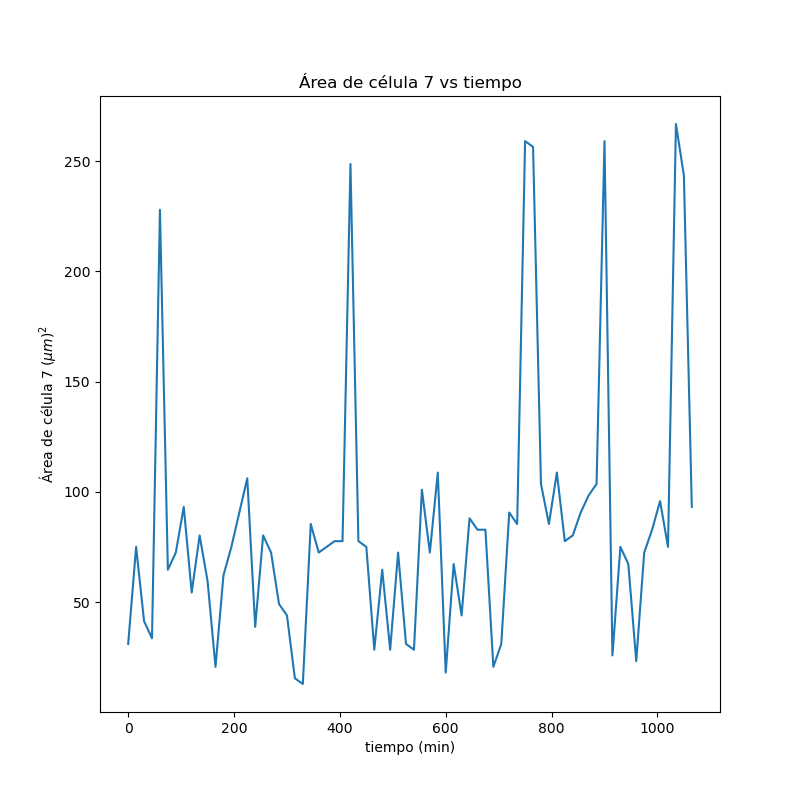
\includegraphics[scale=0.4]{Area_de_celula_7_vs_tiempo.png} 
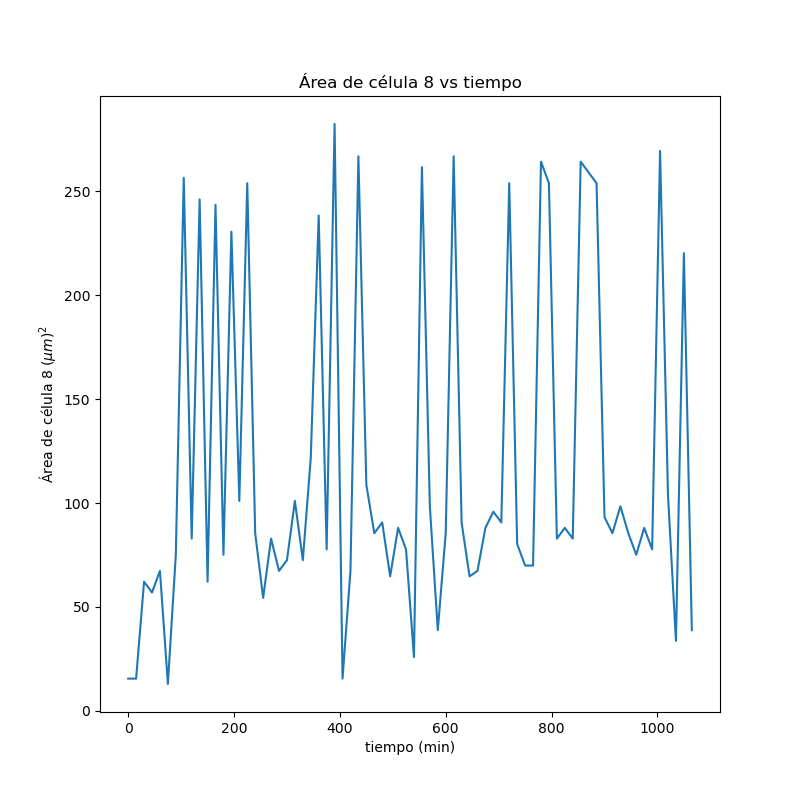
\includegraphics[scale=0.4]{Area_de_celula_8_vs_tiempo.png} 
\\
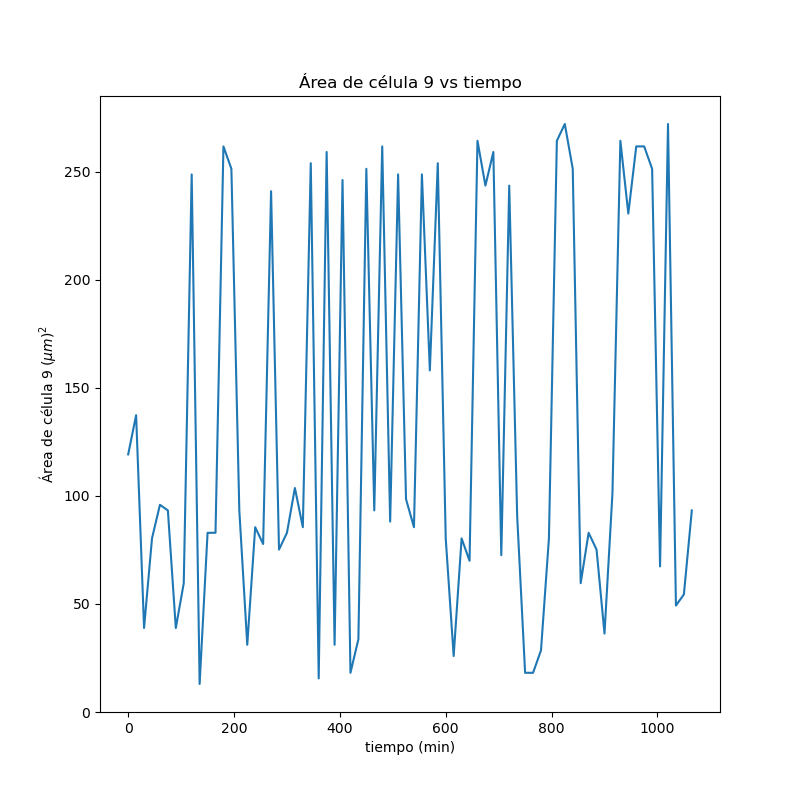
\includegraphics[scale=0.4]{Area_de_celula_9_vs_tiempo.png} 
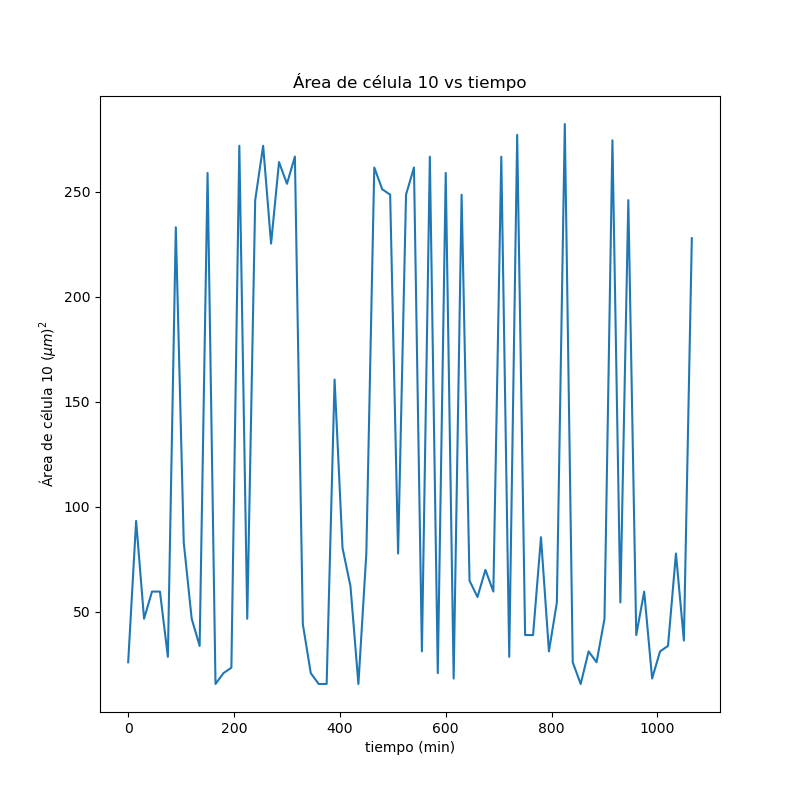
\includegraphics[scale=0.4]{Area_de_celula_10_vs_tiempo.png} 
\\
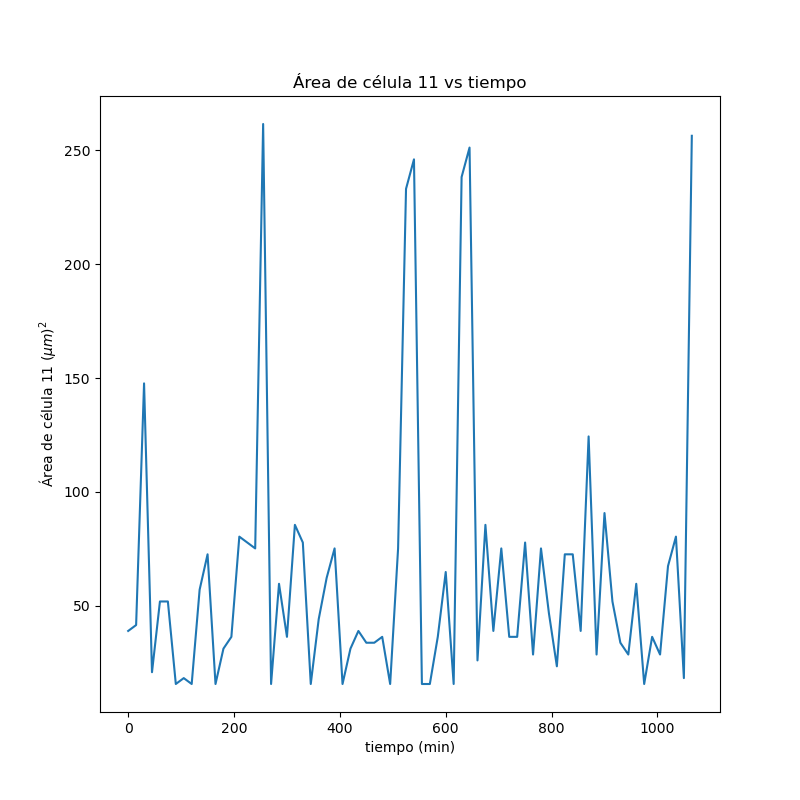
\includegraphics[scale=0.4]{Area_de_celula_11_vs_tiempo.png} 
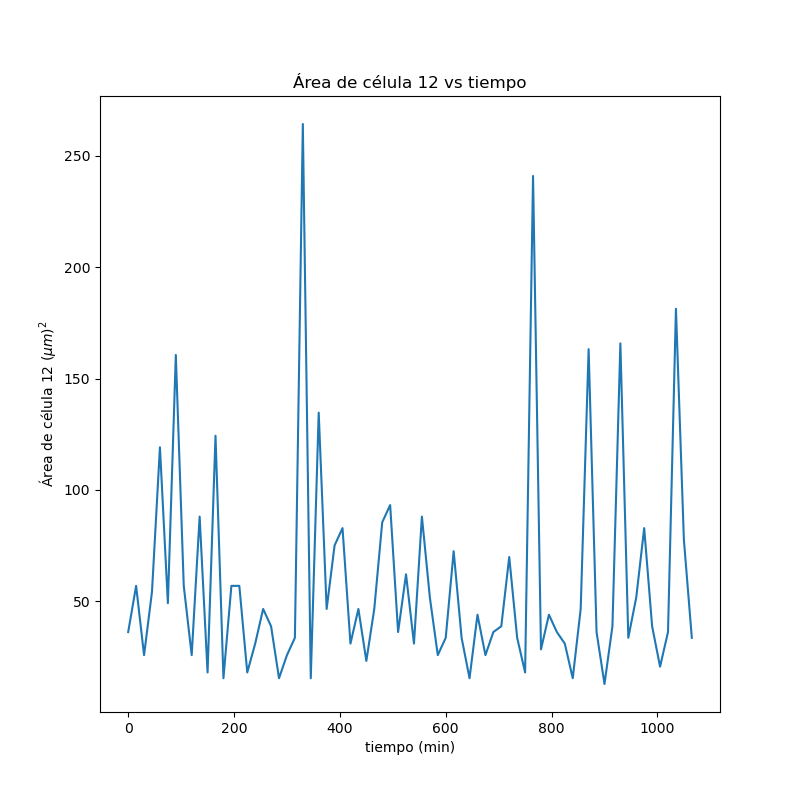
\includegraphics[scale=0.4]{Area_de_celula_12_vs_tiempo.png} 
\\
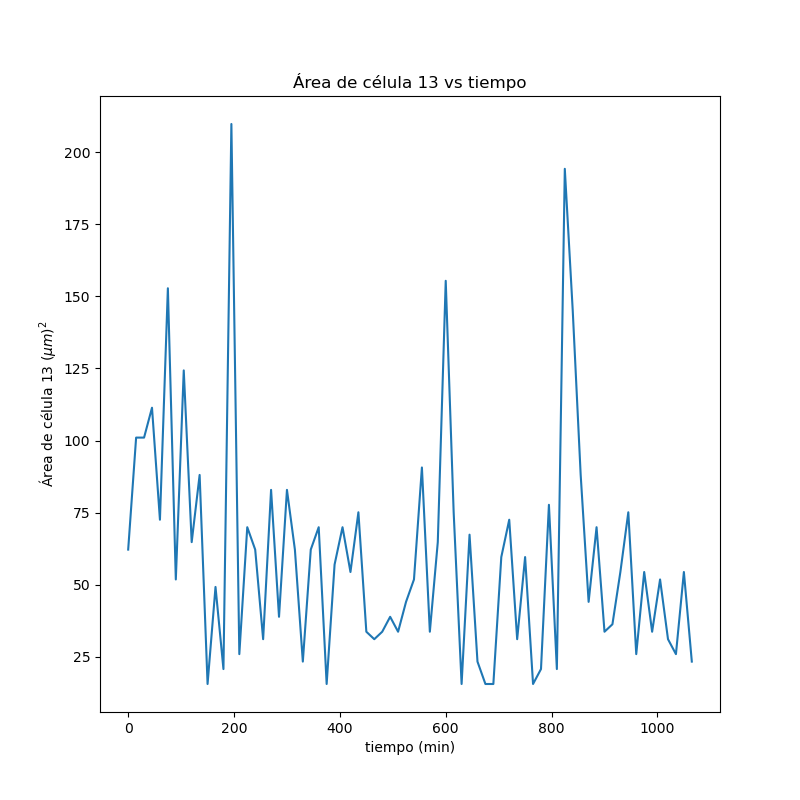
\includegraphics[scale=0.4]{Area_de_celula_13_vs_tiempo.png} 
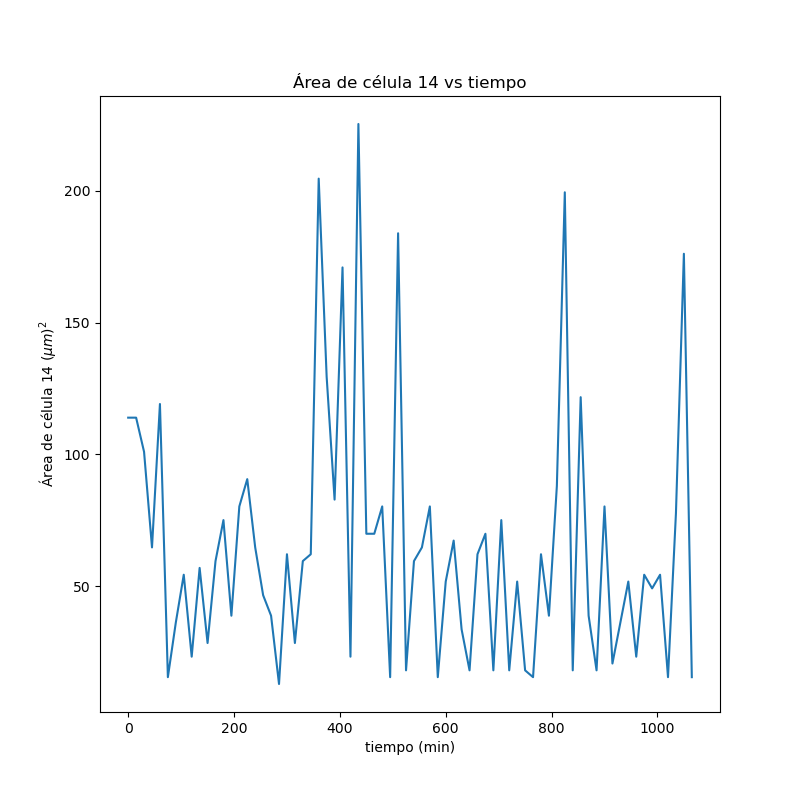
\includegraphics[scale=0.4]{Area_de_celula_14_vs_tiempo.png} 
\\
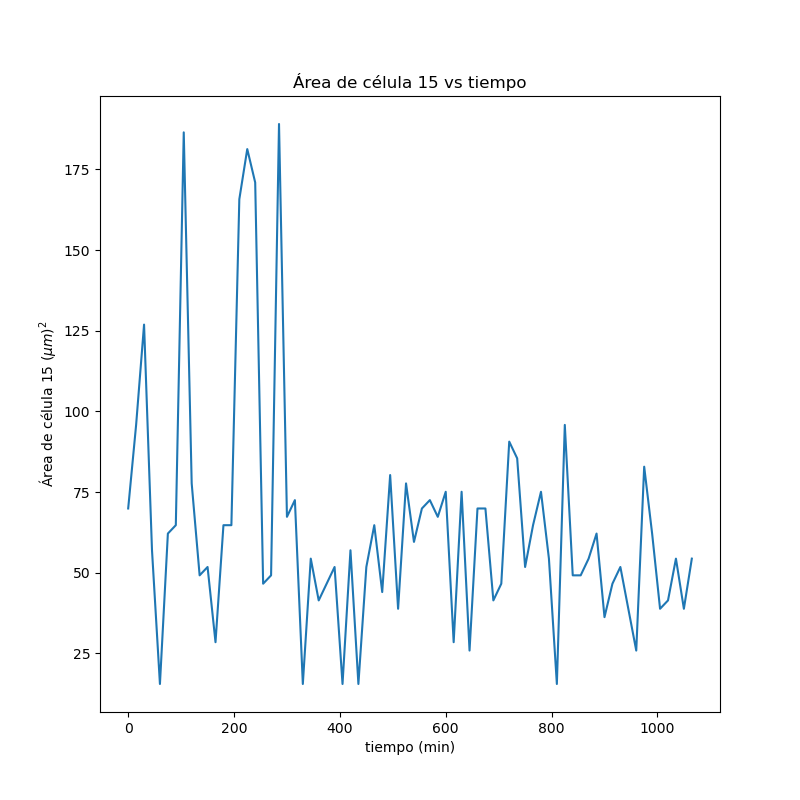
\includegraphics[scale=0.4]{Area_de_celula_15_vs_tiempo.png} 
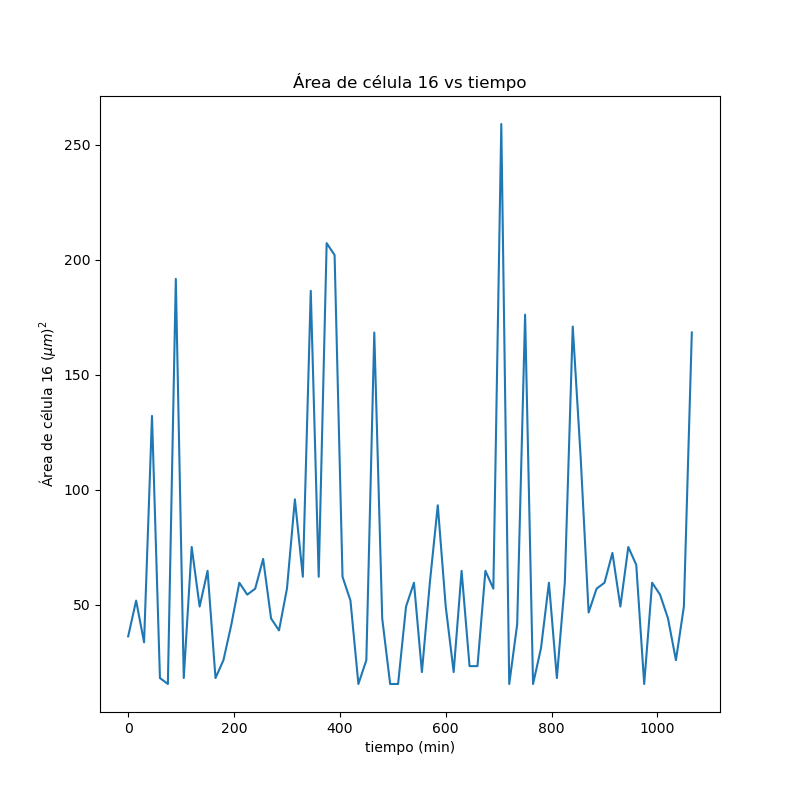
\includegraphics[scale=0.4]{Area_de_celula_16_vs_tiempo.png} 
\\
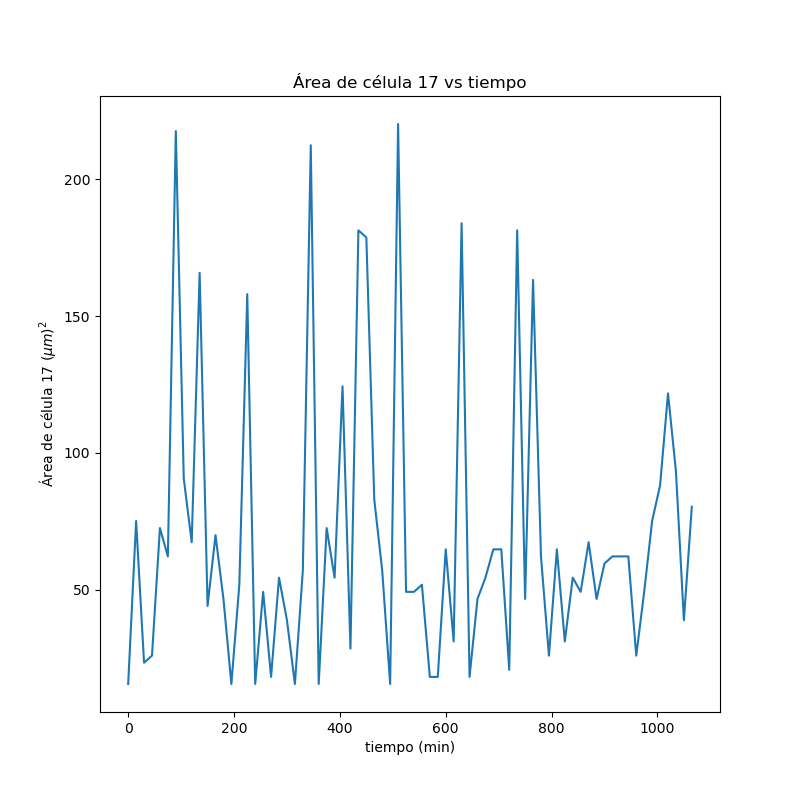
\includegraphics[scale=0.4]{Area_de_celula_17_vs_tiempo.png} 
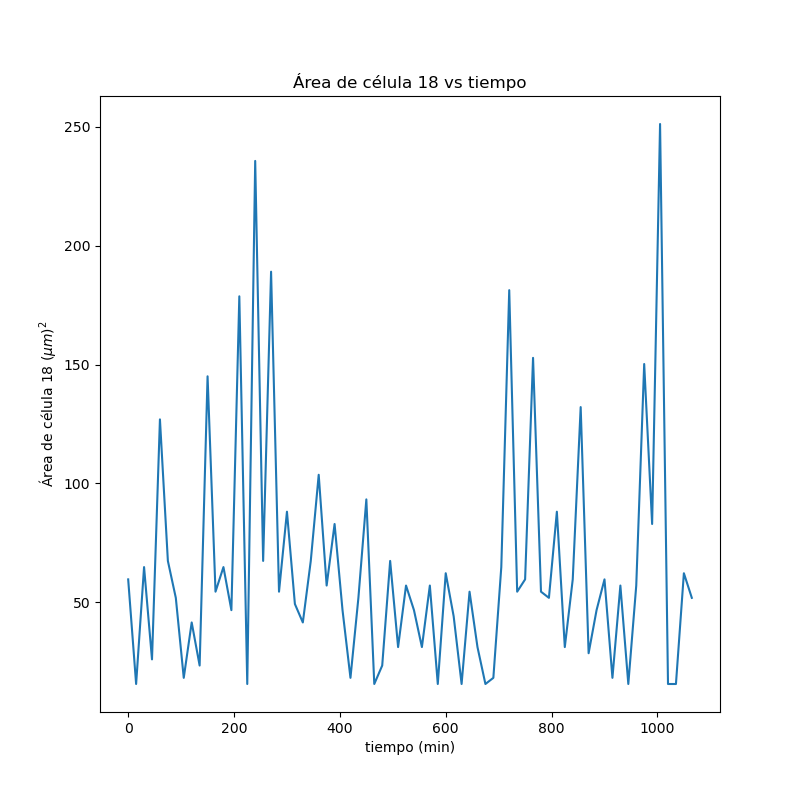
\includegraphics[scale=0.4]{Area_de_celula_18_vs_tiempo.png} 
\\
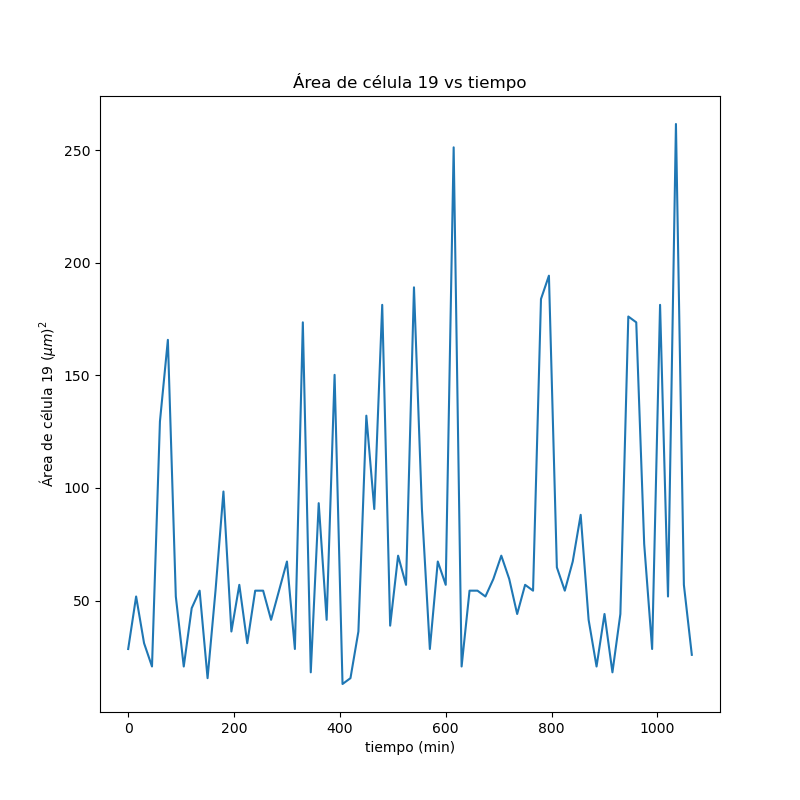
\includegraphics[scale=0.4]{Area_de_celula_19_vs_tiempo.png} 
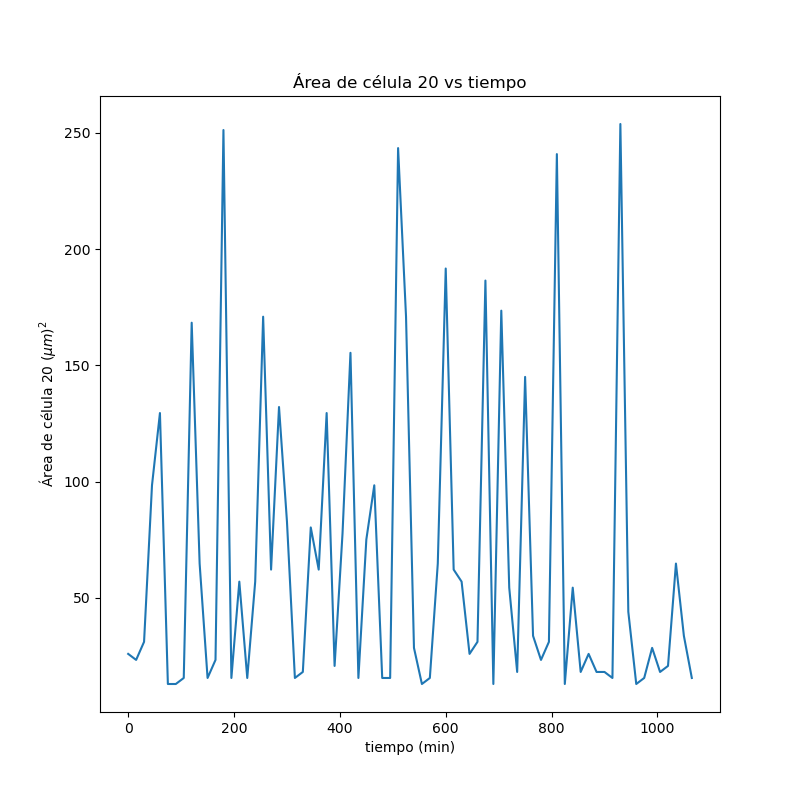
\includegraphics[scale=0.4]{Area_de_celula_20_vs_tiempo.png} 
\\
\newpage
A continuaci\'on se presentan los gr\'aficos de Largo vs tiempo.\\
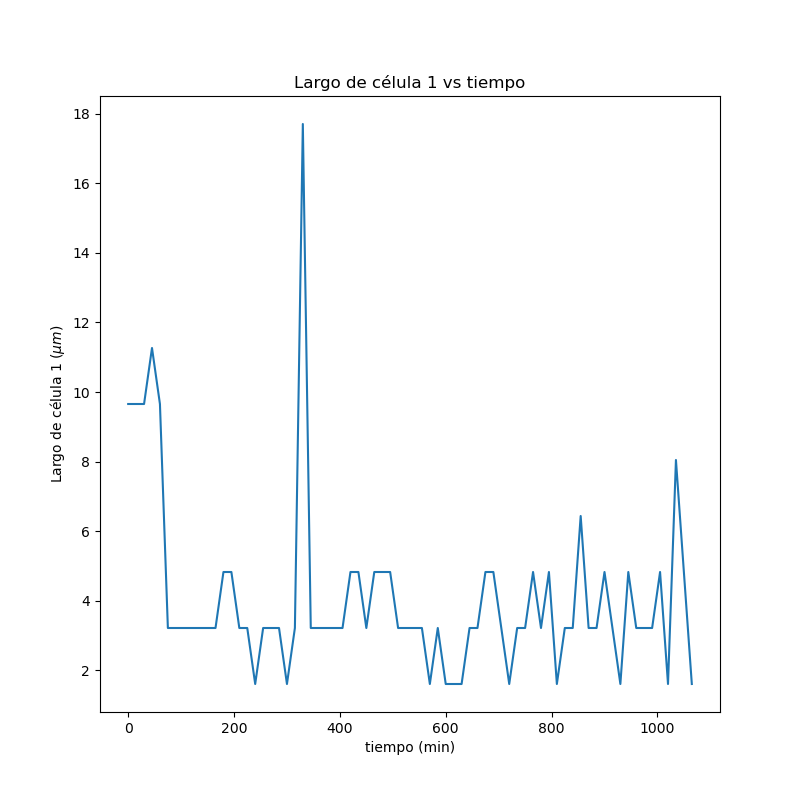
\includegraphics[scale=0.4]{Largo_de_celula_1_vs_tiempo.png} 
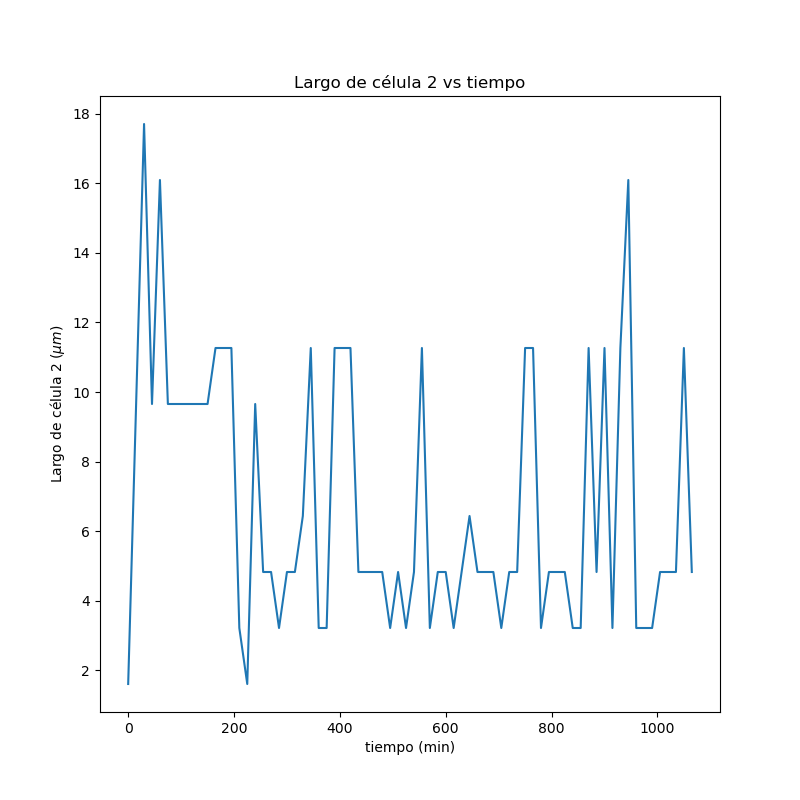
\includegraphics[scale=0.4]{Largo_de_celula_2_vs_tiempo.png} 
\\
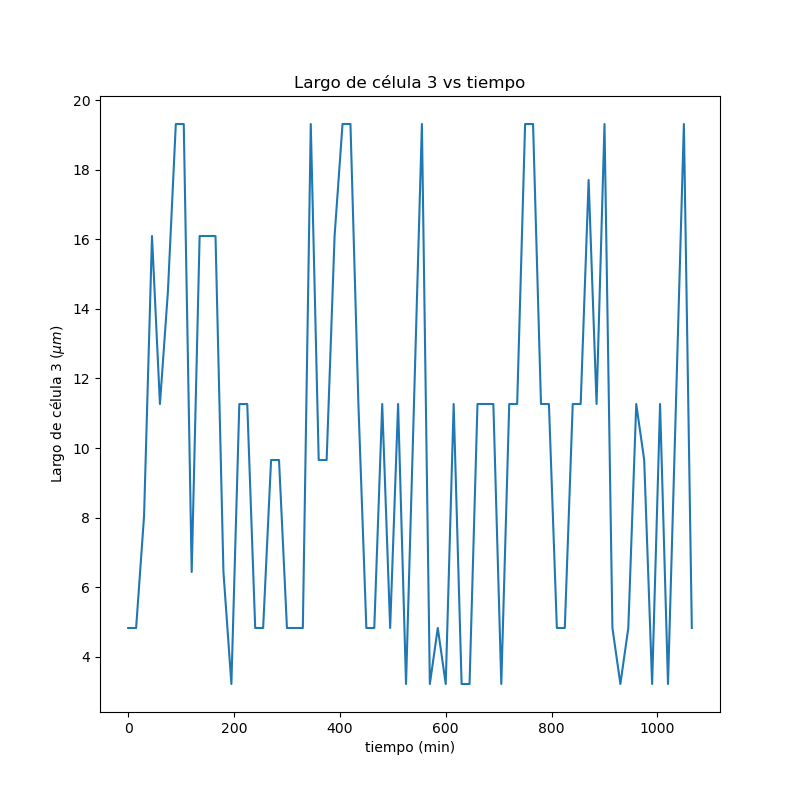
\includegraphics[scale=0.4]{Largo_de_celula_3_vs_tiempo.png} 
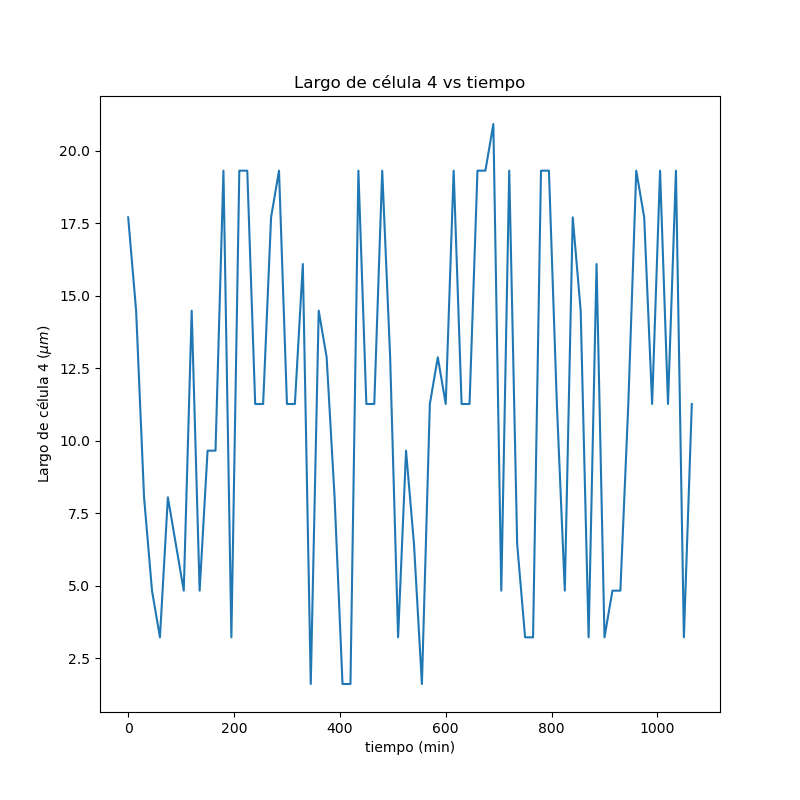
\includegraphics[scale=0.4]{Largo_de_celula_4_vs_tiempo.png} 
\\
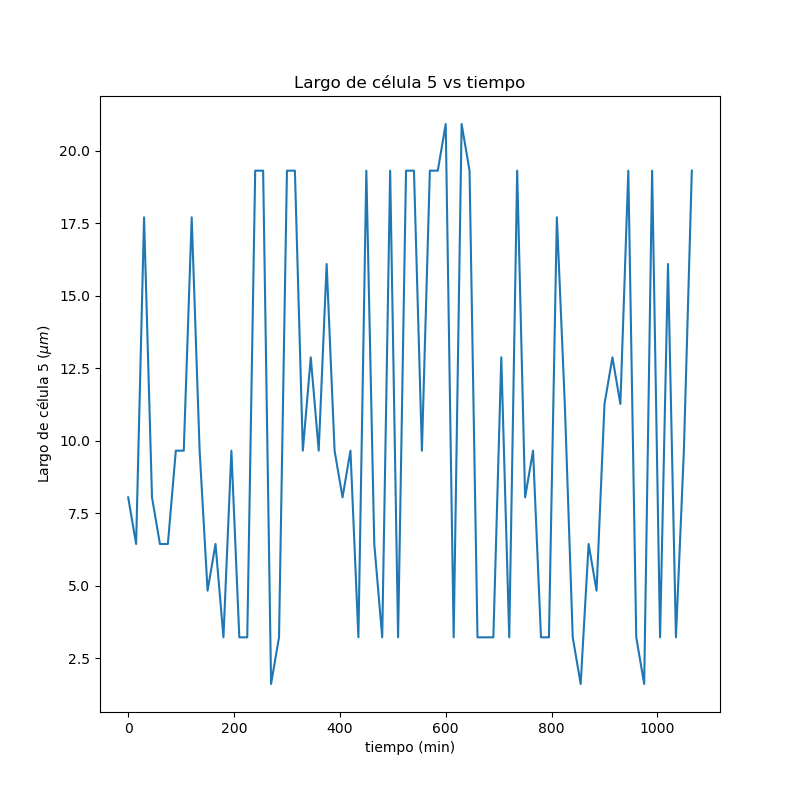
\includegraphics[scale=0.4]{Largo_de_celula_5_vs_tiempo.png} 
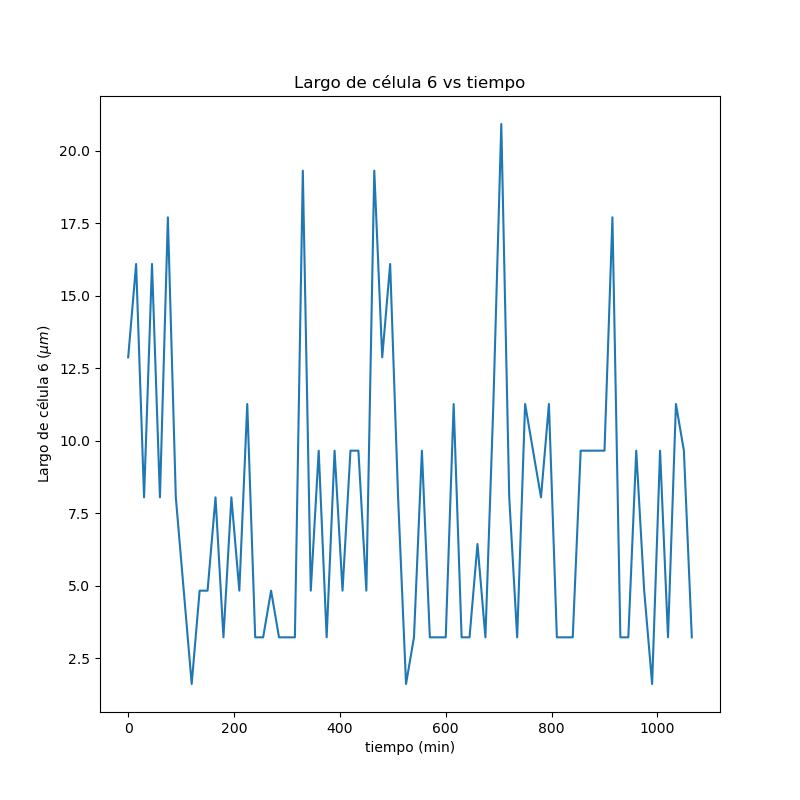
\includegraphics[scale=0.4]{Largo_de_celula_6_vs_tiempo.png} 
\\
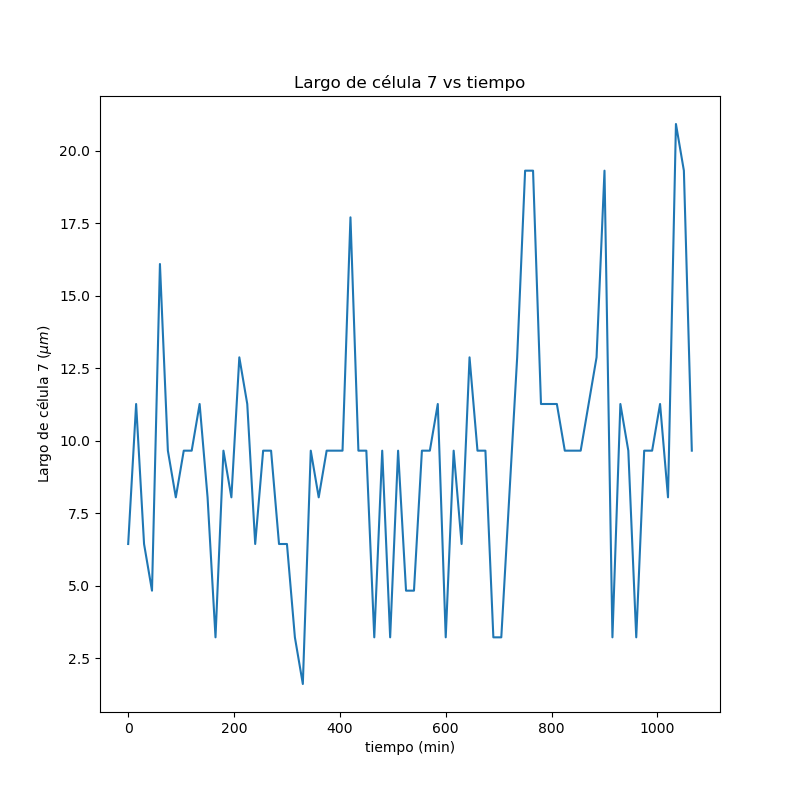
\includegraphics[scale=0.4]{Largo_de_celula_7_vs_tiempo.png} 
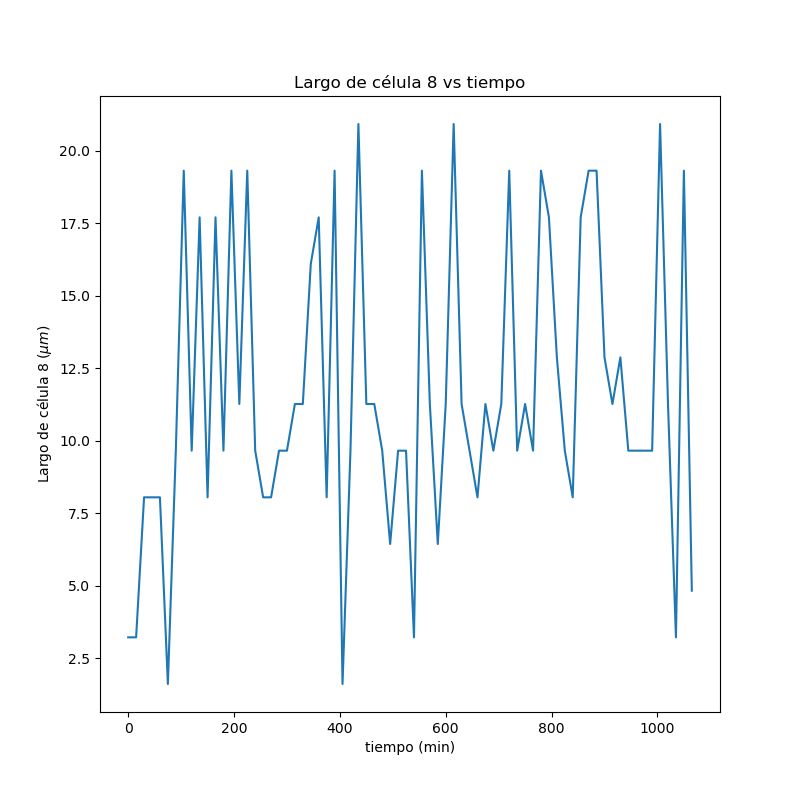
\includegraphics[scale=0.4]{Largo_de_celula_8_vs_tiempo.png} 
\\
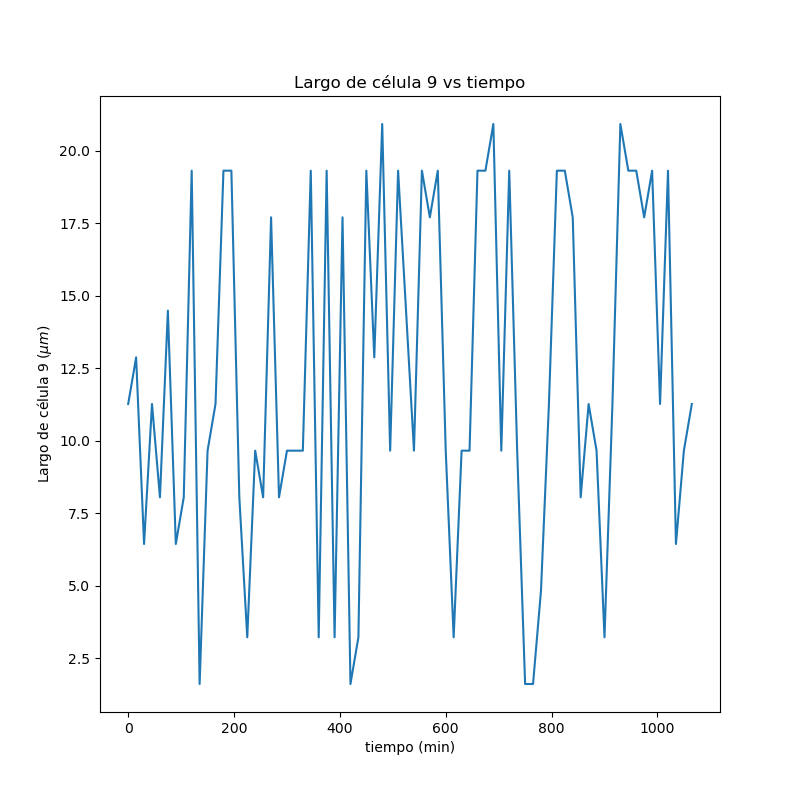
\includegraphics[scale=0.4]{Largo_de_celula_9_vs_tiempo.png} 
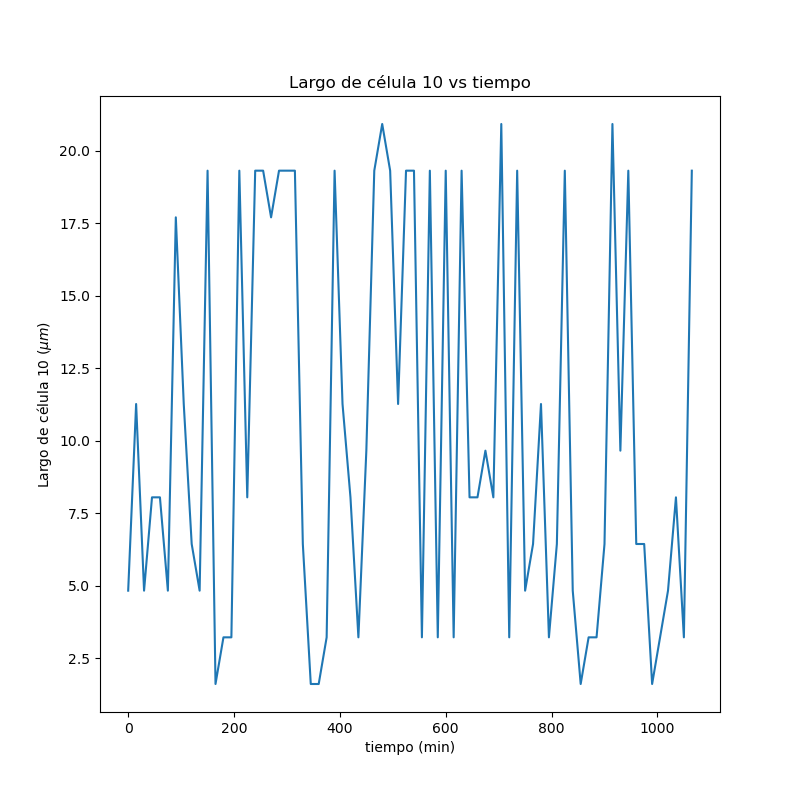
\includegraphics[scale=0.4]{Largo_de_celula_10_vs_tiempo.png} 
\\
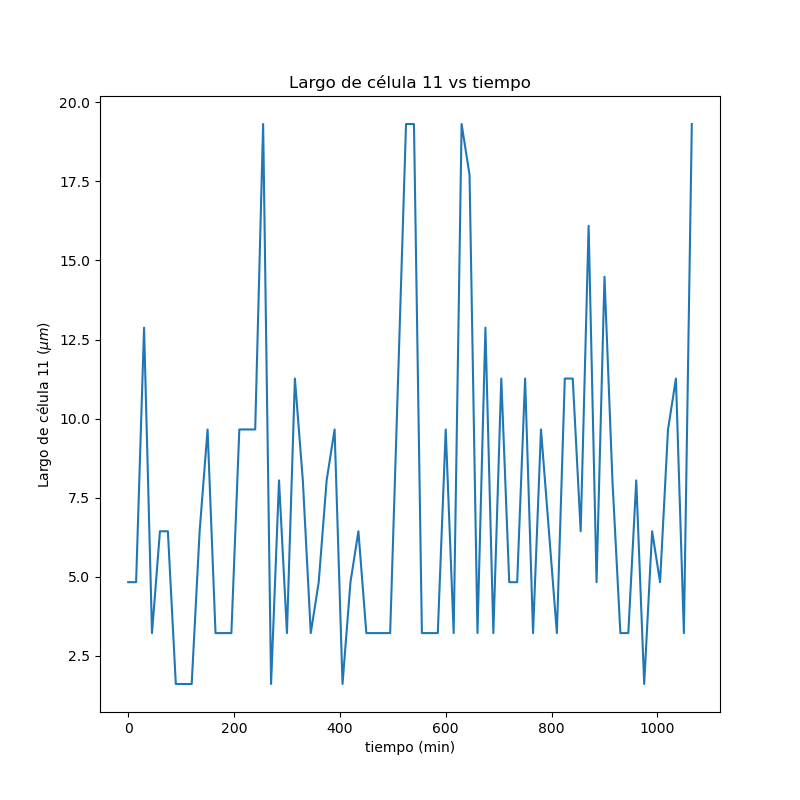
\includegraphics[scale=0.4]{Largo_de_celula_11_vs_tiempo.png} 
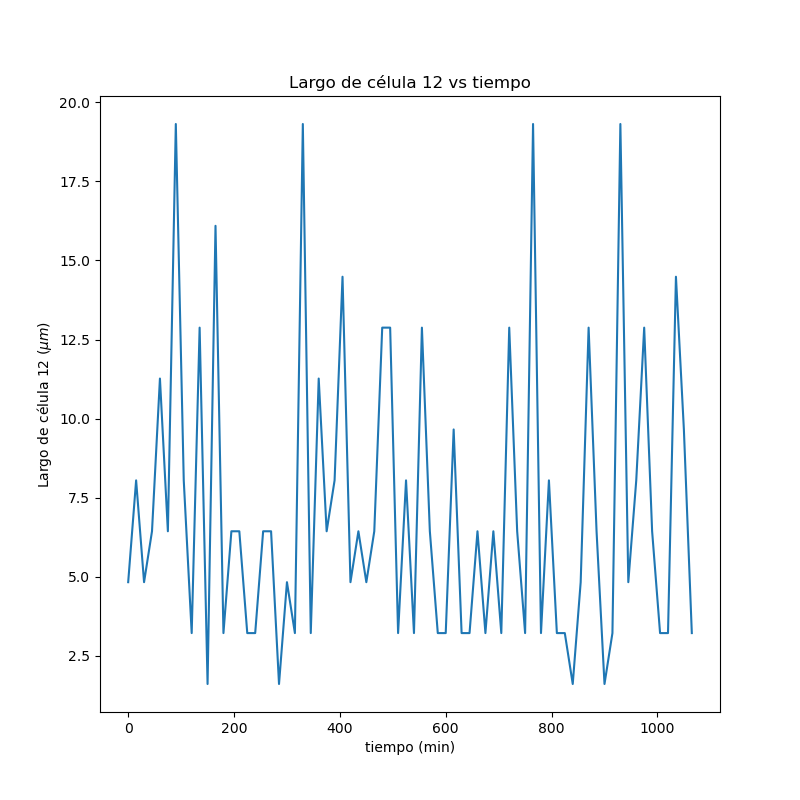
\includegraphics[scale=0.4]{Largo_de_celula_12_vs_tiempo.png} 
\\
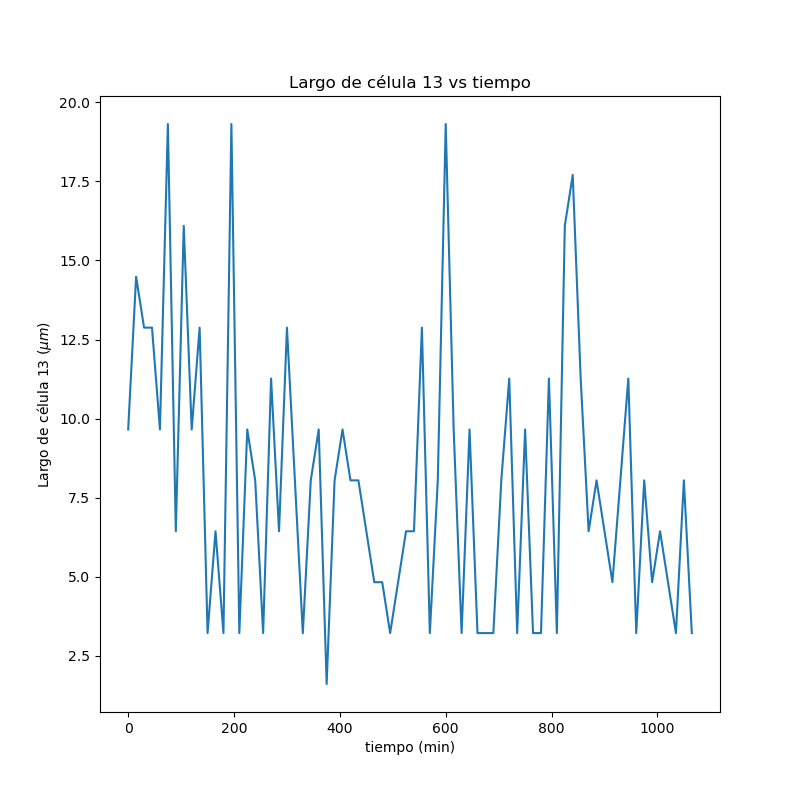
\includegraphics[scale=0.4]{Largo_de_celula_13_vs_tiempo.png} 
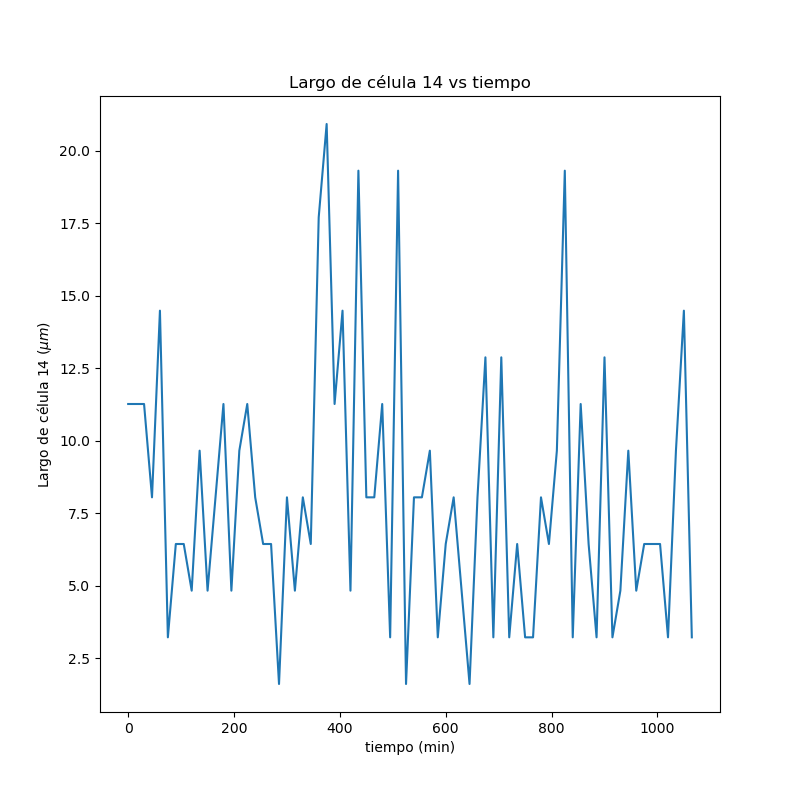
\includegraphics[scale=0.4]{Largo_de_celula_14_vs_tiempo.png} 
\\
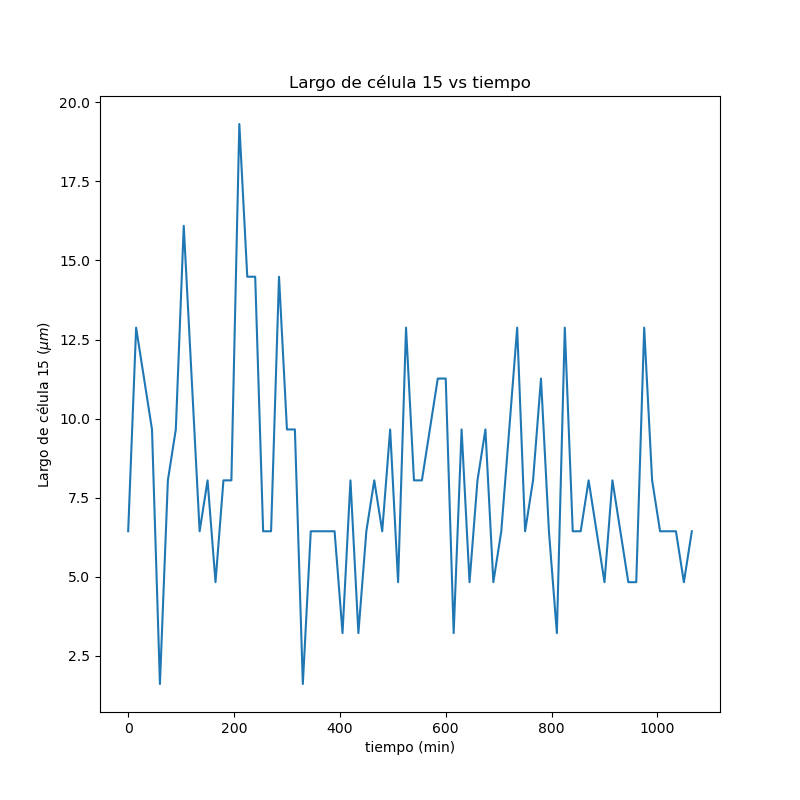
\includegraphics[scale=0.4]{Largo_de_celula_15_vs_tiempo.png} 
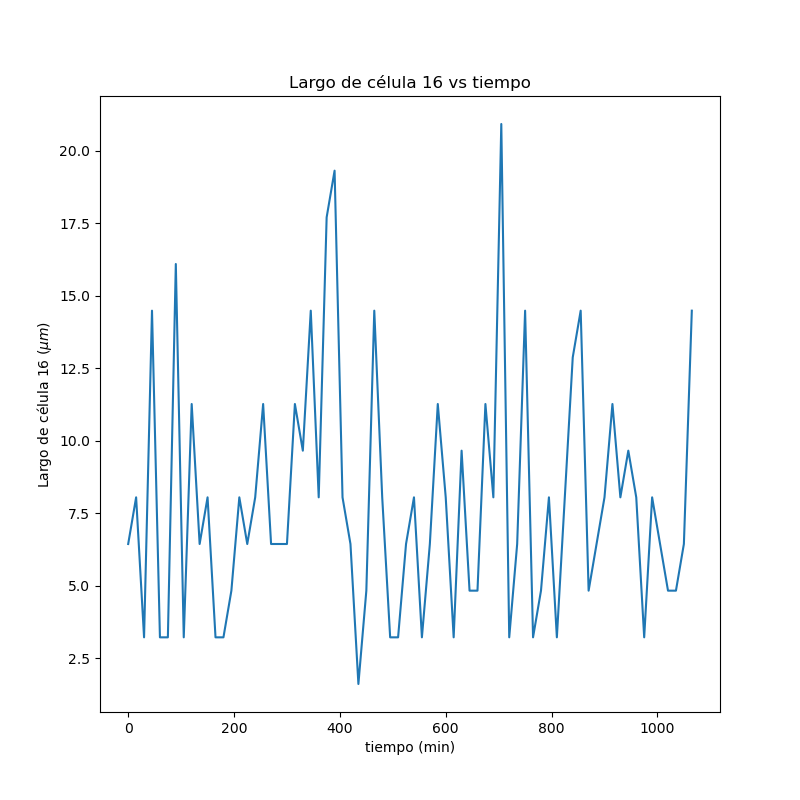
\includegraphics[scale=0.4]{Largo_de_celula_16_vs_tiempo.png} 
\\
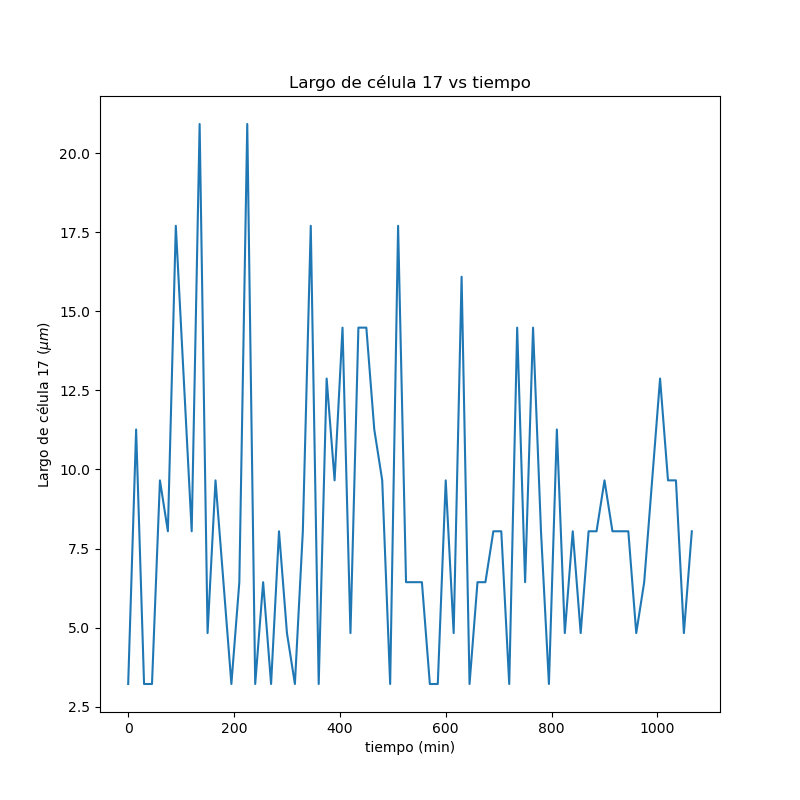
\includegraphics[scale=0.4]{Largo_de_celula_17_vs_tiempo.png} 
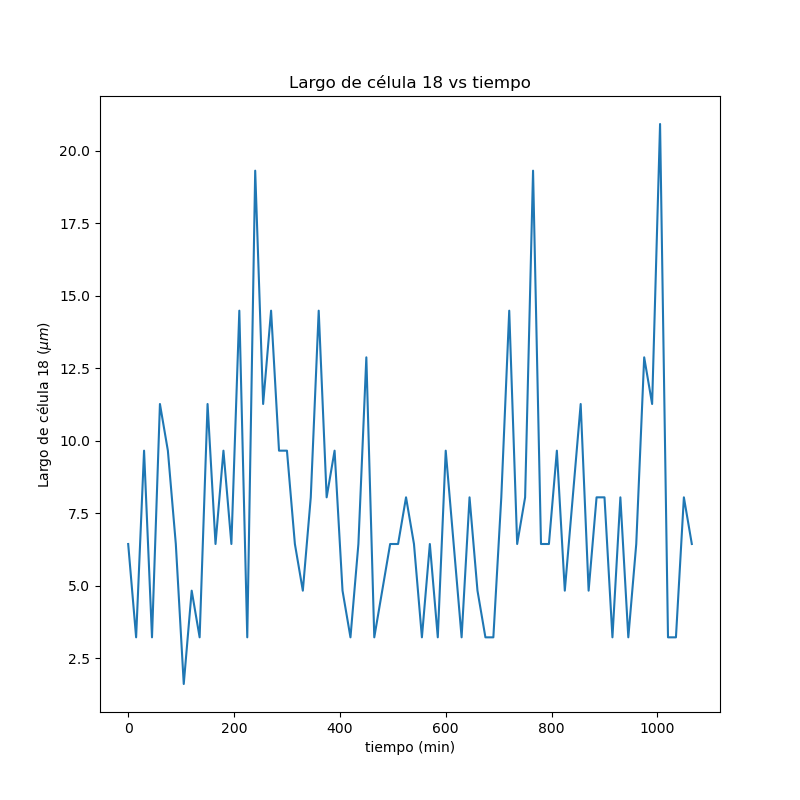
\includegraphics[scale=0.4]{Largo_de_celula_18_vs_tiempo.png} 
\\
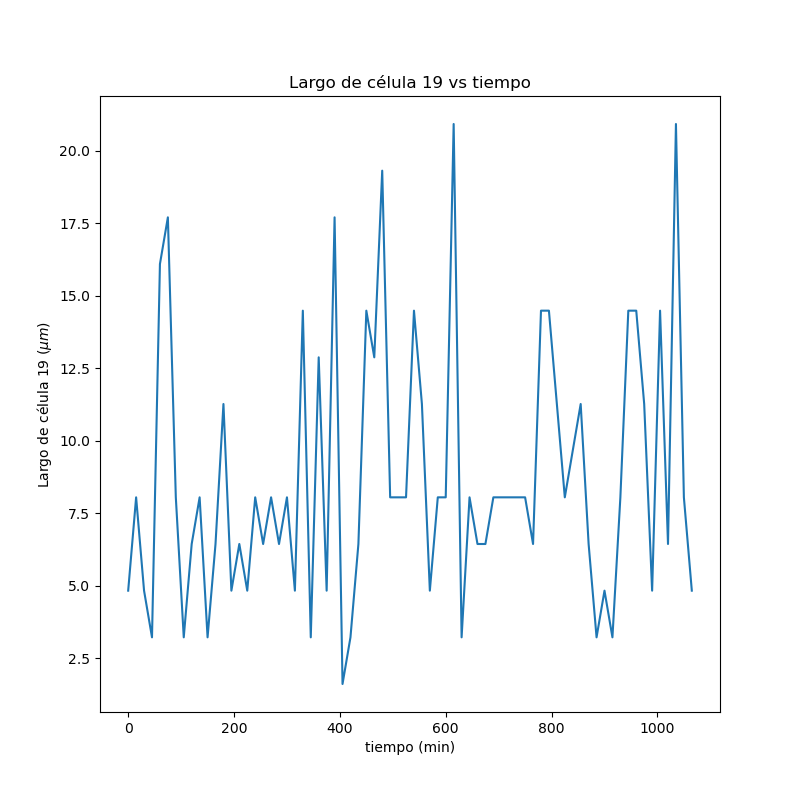
\includegraphics[scale=0.4]{Largo_de_celula_19_vs_tiempo.png} 
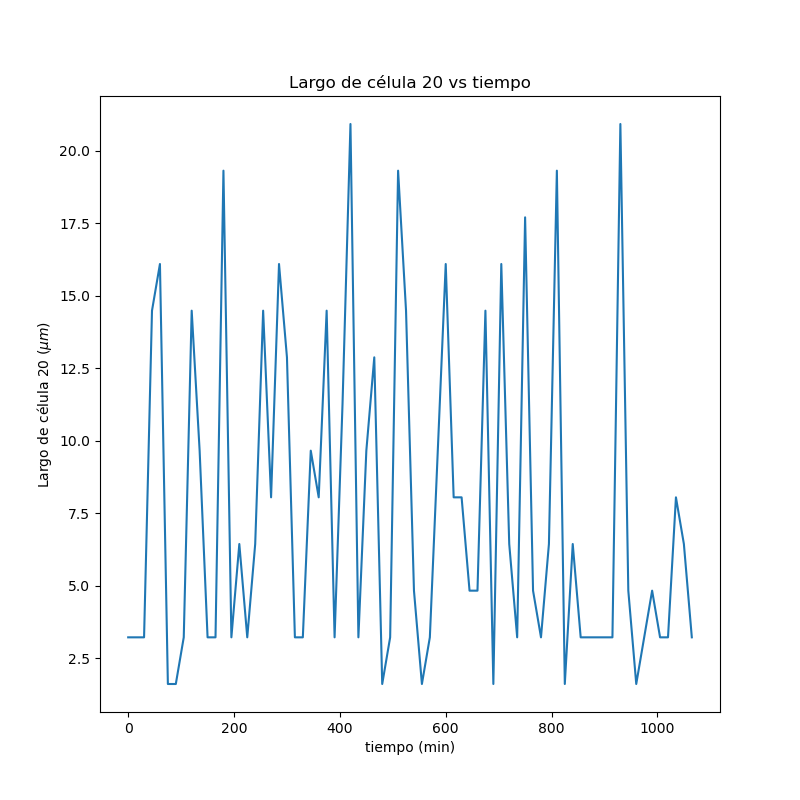
\includegraphics[scale=0.4]{Largo_de_celula_20_vs_tiempo.png} 
\\
\newpage
A continuaci\'on se presentan los gr\'aficos de Alto vs tiempo.\\
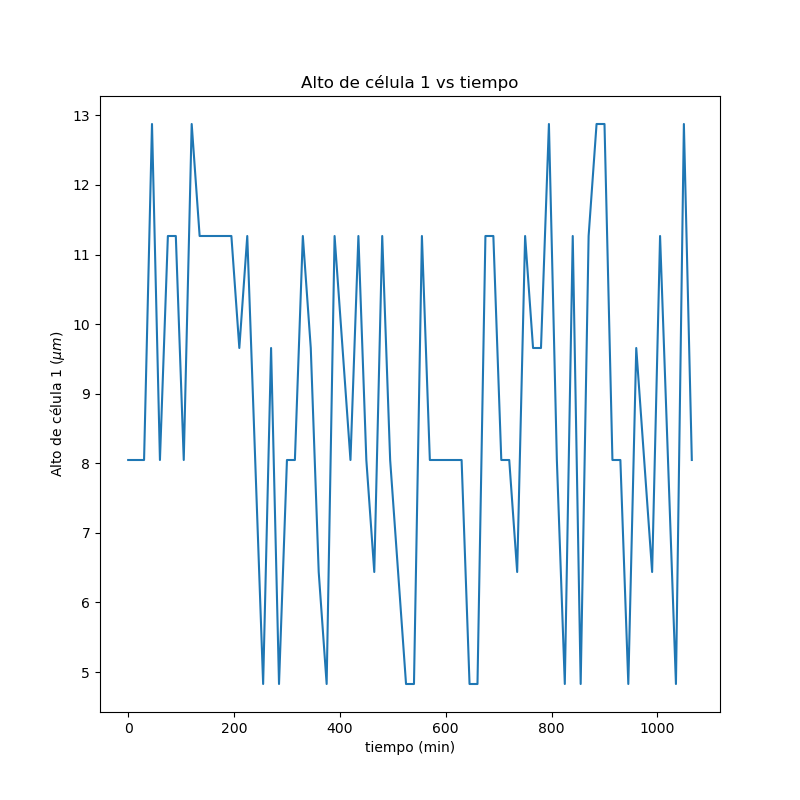
\includegraphics[scale=0.4]{Alto_de_celula_1_vs_tiempo.png} 
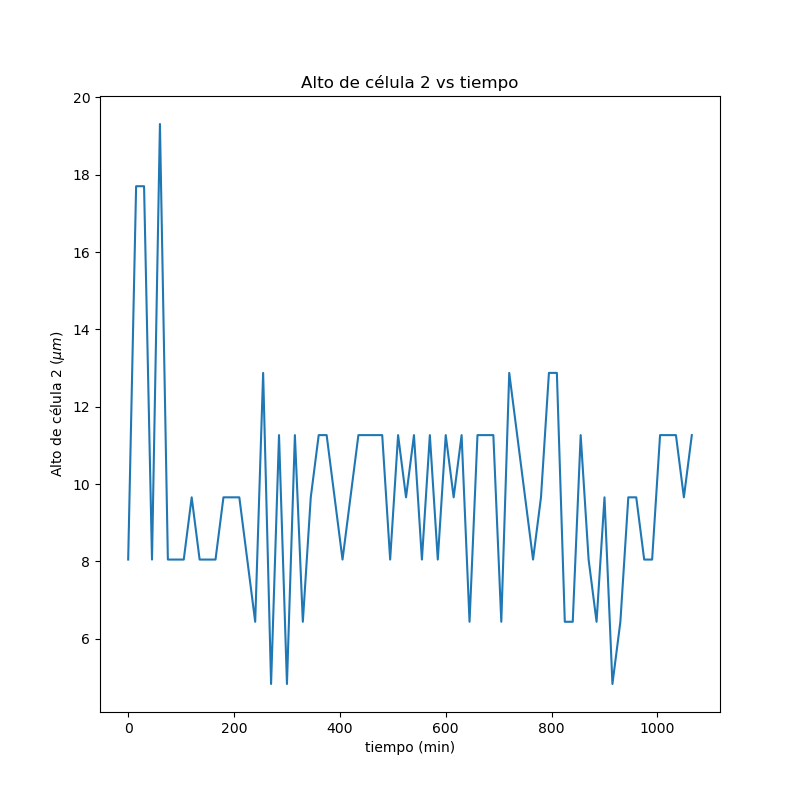
\includegraphics[scale=0.4]{Alto_de_celula_2_vs_tiempo.png} 
\\
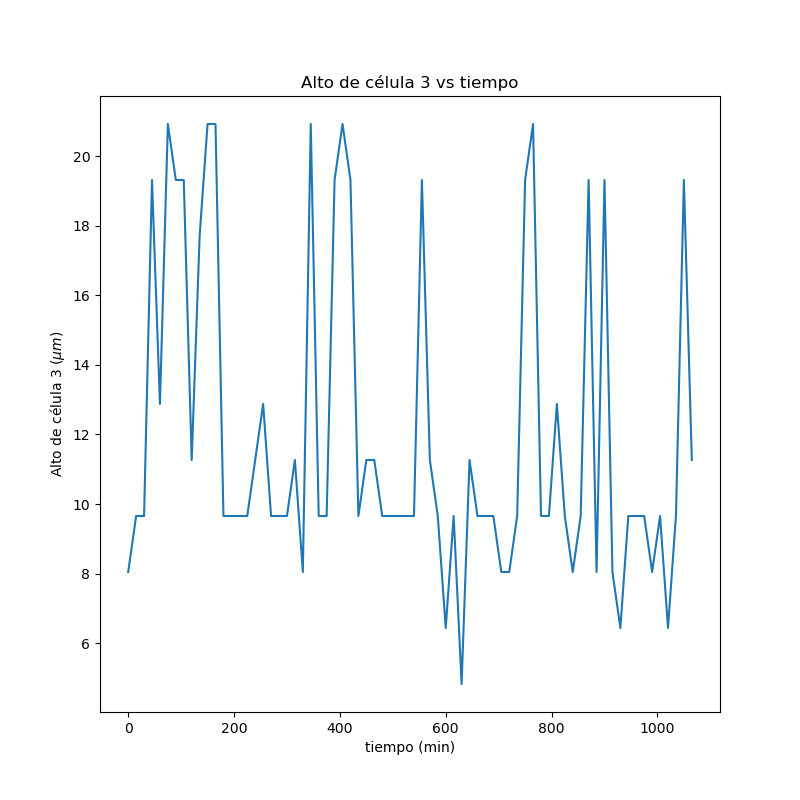
\includegraphics[scale=0.4]{Alto_de_celula_3_vs_tiempo.png} 
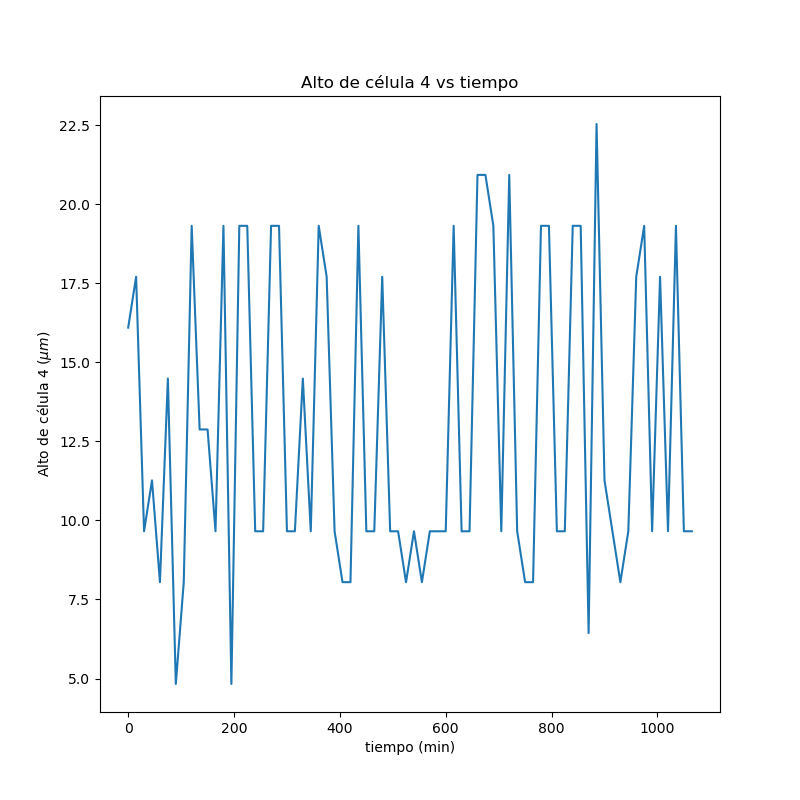
\includegraphics[scale=0.4]{Alto_de_celula_4_vs_tiempo.png} 
\\
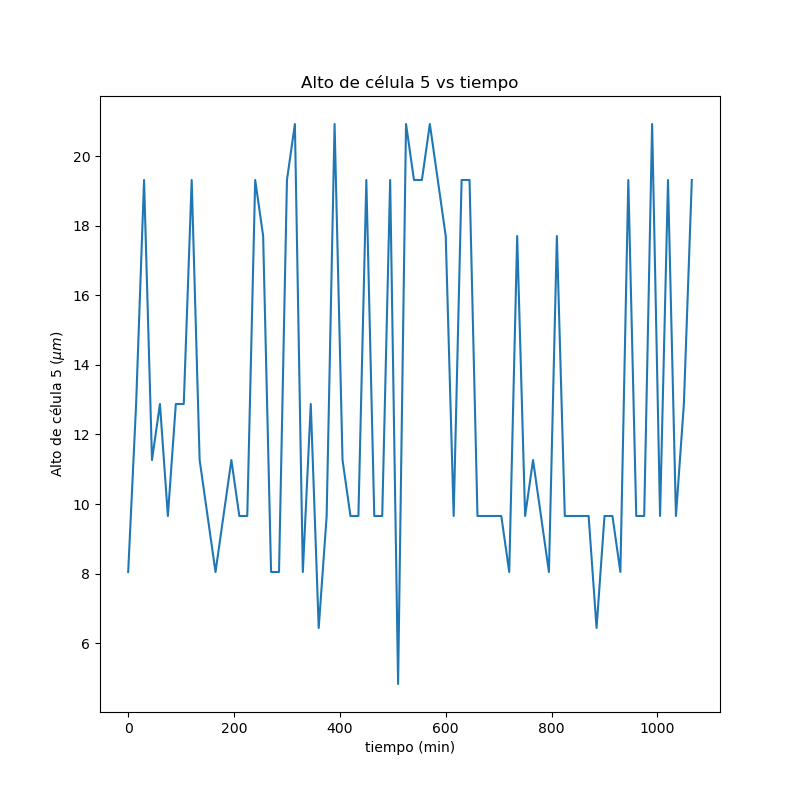
\includegraphics[scale=0.4]{Alto_de_celula_5_vs_tiempo.png} 
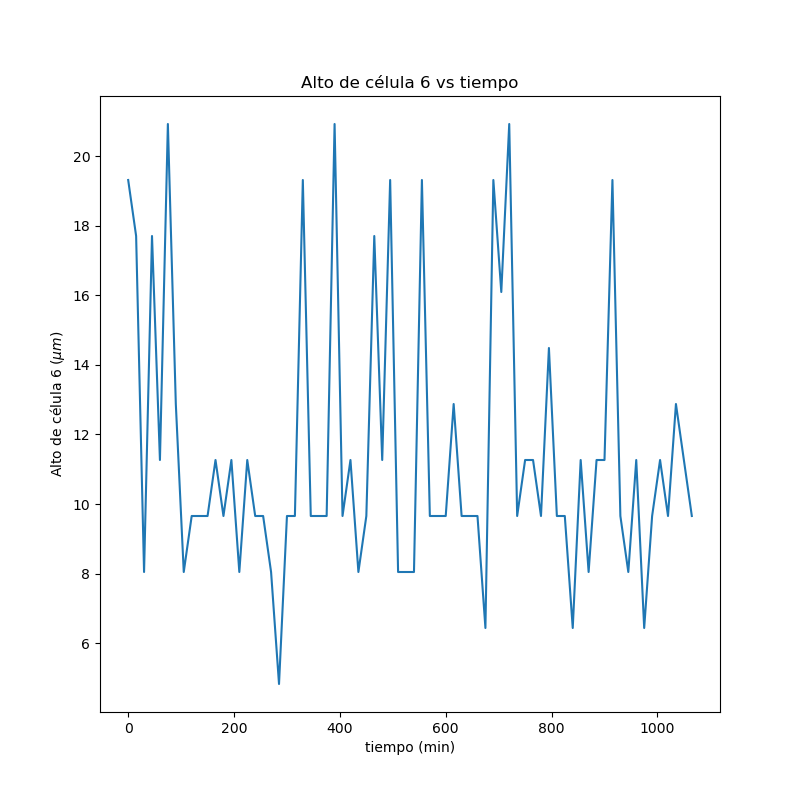
\includegraphics[scale=0.4]{Alto_de_celula_6_vs_tiempo.png} 
\\
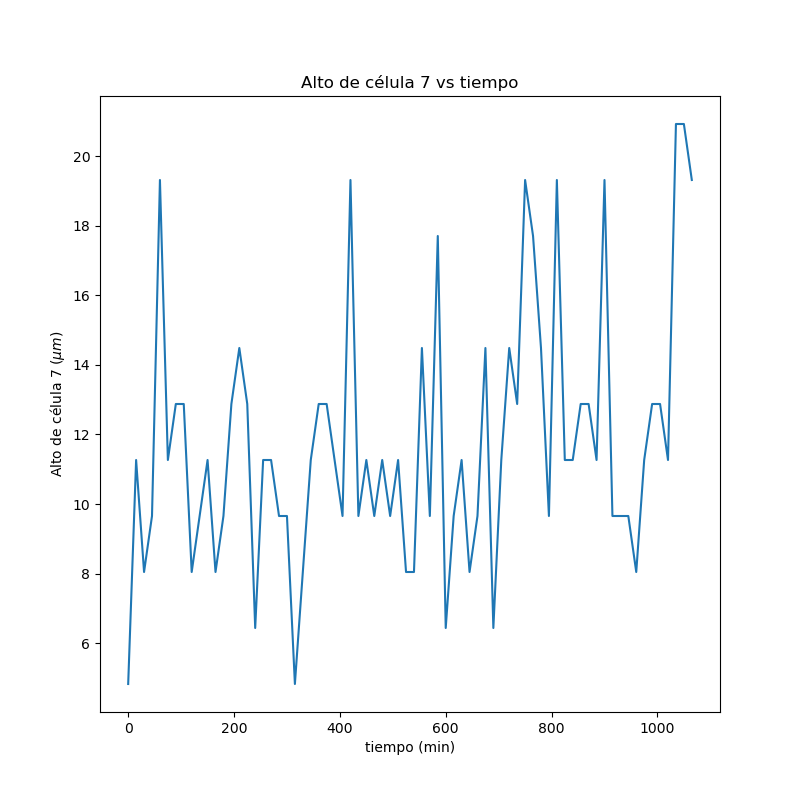
\includegraphics[scale=0.4]{Alto_de_celula_7_vs_tiempo.png} 
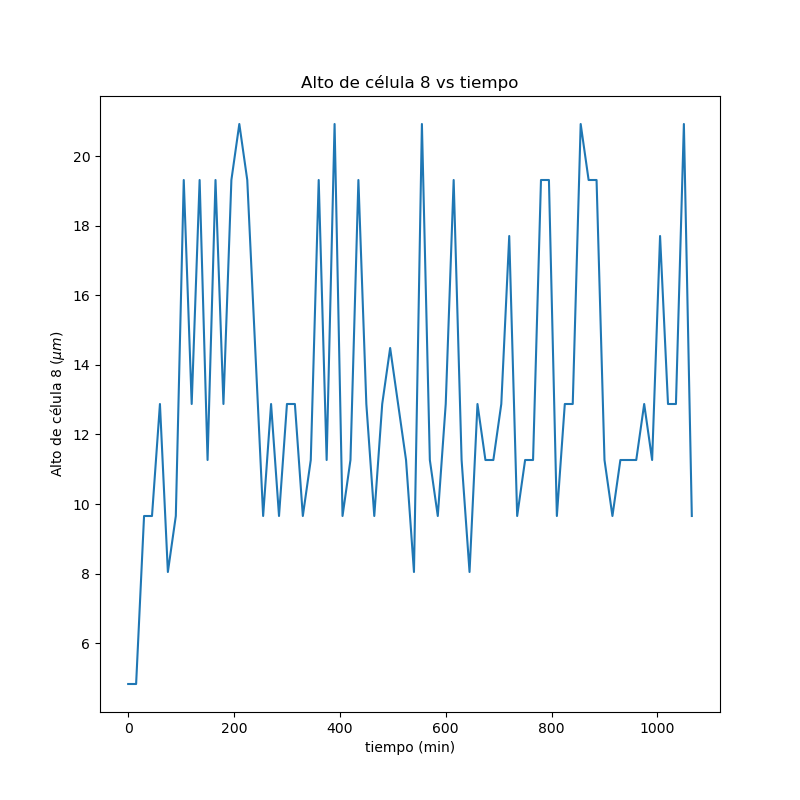
\includegraphics[scale=0.4]{Alto_de_celula_8_vs_tiempo.png} 
\\
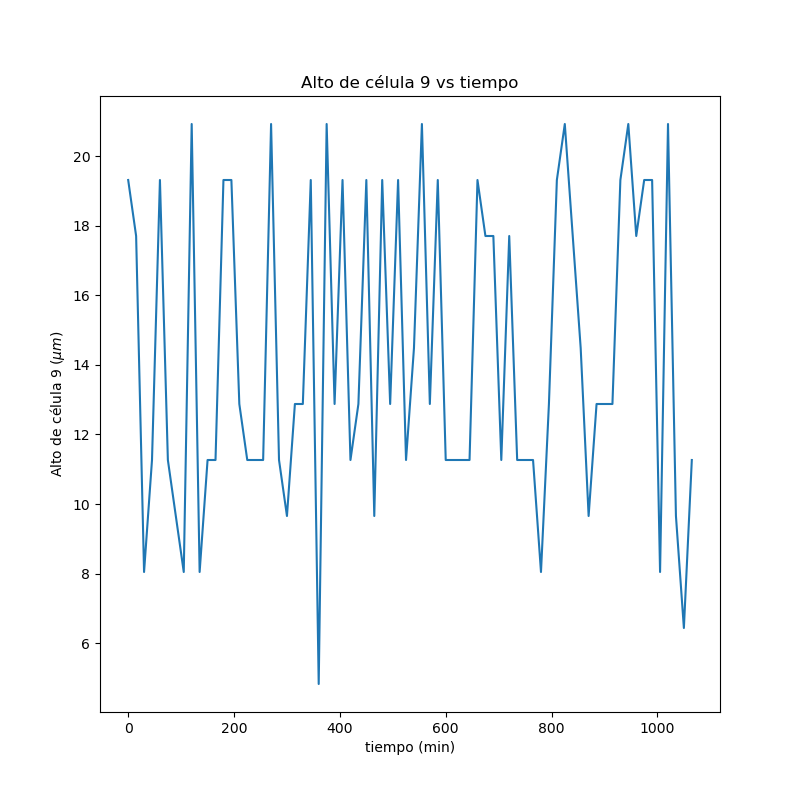
\includegraphics[scale=0.4]{Alto_de_celula_9_vs_tiempo.png} 
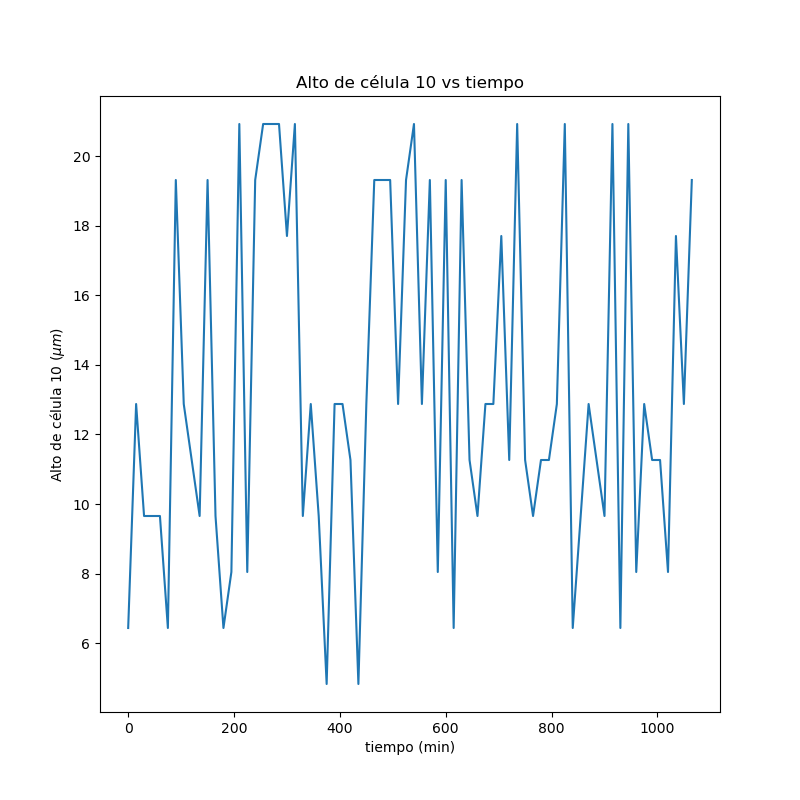
\includegraphics[scale=0.4]{Alto_de_celula_10_vs_tiempo.png} 
\\
\includegraphics[scale=0.4]{Alto_de_celula_11_vs_tiempo.png} 
\includegraphics[scale=0.4]{Alto_de_celula_12_vs_tiempo.png} 
\\
\includegraphics[scale=0.4]{Alto_de_celula_13_vs_tiempo.png} 
\includegraphics[scale=0.4]{Alto_de_celula_14_vs_tiempo.png} 
\\
\includegraphics[scale=0.4]{Alto_de_celula_15_vs_tiempo.png} 
\includegraphics[scale=0.4]{Alto_de_celula_16_vs_tiempo.png} 
\\
\includegraphics[scale=0.4]{Alto_de_celula_17_vs_tiempo.png} 
\includegraphics[scale=0.4]{Alto_de_celula_18_vs_tiempo.png} 
\\
\includegraphics[scale=0.4]{Alto_de_celula_19_vs_tiempo.png} 
\includegraphics[scale=0.4]{Alto_de_celula_20_vs_tiempo.png} 
\\
\newpage
A continuaci\'on se presentan los gr\'aficos de velocidades vs tiempo.\\
\includegraphics[scale=0.4]{Velocidad_de_celula_1.png} 
\includegraphics[scale=0.4]{Velocidad_de_celula_2.png} 
\\
\includegraphics[scale=0.4]{Velocidad_de_celula_3.png} 
\includegraphics[scale=0.4]{Velocidad_de_celula_4.png} 
\\
\includegraphics[scale=0.4]{Velocidad_de_celula_5.png} 
\includegraphics[scale=0.4]{Velocidad_de_celula_6.png} 
\\
\includegraphics[scale=0.4]{Velocidad_de_celula_7.png} 
\includegraphics[scale=0.4]{Velocidad_de_celula_8.png} 
\\
\includegraphics[scale=0.4]{Velocidad_de_celula_9.png} 
\includegraphics[scale=0.4]{Velocidad_de_celula_10.png} 
\\
\includegraphics[scale=0.4]{Velocidad_de_celula_11.png} 
\includegraphics[scale=0.4]{Velocidad_de_celula_12.png} 
\\
\includegraphics[scale=0.4]{Velocidad_de_celula_13.png} 
\includegraphics[scale=0.4]{Velocidad_de_celula_14.png} 
\\
\includegraphics[scale=0.4]{Velocidad_de_celula_15.png} 
\includegraphics[scale=0.4]{Velocidad_de_celula_16.png} 
\\
\includegraphics[scale=0.4]{Velocidad_de_celula_17.png} 
\includegraphics[scale=0.4]{Velocidad_de_celula_18.png} 
\\
\includegraphics[scale=0.4]{Velocidad_de_celula_19.png} 
\includegraphics[scale=0.4]{Velocidad_de_celula_20.png} 
\\
\newpage
A continuaci\'on se presentan los gr\'aficos de variaciones del \'Area vs tiempo\\
\includegraphics[scale=0.4]{Variacion_de_Area_de_celula_1.png} 
\includegraphics[scale=0.4]{Variacion_de_Area_de_celula_2.png} 
\\
\includegraphics[scale=0.4]{Variacion_de_Area_de_celula_3.png} 
\includegraphics[scale=0.4]{Variacion_de_Area_de_celula_4.png} 
\\
\includegraphics[scale=0.4]{Variacion_de_Area_de_celula_5.png} 
\includegraphics[scale=0.4]{Variacion_de_Area_de_celula_6.png} 
\\
\includegraphics[scale=0.4]{Variacion_de_Area_de_celula_7.png} 
\includegraphics[scale=0.4]{Variacion_de_Area_de_celula_8.png} 
\\
\includegraphics[scale=0.4]{Variacion_de_Area_de_celula_9.png} 
\includegraphics[scale=0.4]{Variacion_de_Area_de_celula_10.png} 
\\
\includegraphics[scale=0.4]{Variacion_de_Area_de_celula_11.png} 
\includegraphics[scale=0.4]{Variacion_de_Area_de_celula_12.png} 
\\
\includegraphics[scale=0.4]{Variacion_de_Area_de_celula_13.png} 
\includegraphics[scale=0.4]{Variacion_de_Area_de_celula_14.png} 
\\
\includegraphics[scale=0.4]{Variacion_de_Area_de_celula_15.png} 
\includegraphics[scale=0.4]{Variacion_de_Area_de_celula_16.png} 
\\
\includegraphics[scale=0.4]{Variacion_de_Area_de_celula_17.png} 
\includegraphics[scale=0.4]{Variacion_de_Area_de_celula_18.png} 
\\
\includegraphics[scale=0.4]{Variacion_de_Area_de_celula_19.png} 
\includegraphics[scale=0.4]{Variacion_de_Area_de_celula_20.png} 
\\
\newpage
A continuaci\'on se presentan los gr\'aficos de variaciones del Largo vs tiempo\\
\includegraphics[scale=0.4]{Variacion_de_Largo_de_celula_1.png} 
\includegraphics[scale=0.4]{Variacion_de_Largo_de_celula_2.png} 
\\
\includegraphics[scale=0.4]{Variacion_de_Largo_de_celula_3.png} 
\includegraphics[scale=0.4]{Variacion_de_Largo_de_celula_4.png} 
\\
\includegraphics[scale=0.4]{Variacion_de_Largo_de_celula_5.png} 
\includegraphics[scale=0.4]{Variacion_de_Largo_de_celula_6.png} 
\\
\includegraphics[scale=0.4]{Variacion_de_Largo_de_celula_7.png} 
\includegraphics[scale=0.4]{Variacion_de_Largo_de_celula_8.png} 
\\
\includegraphics[scale=0.4]{Variacion_de_Largo_de_celula_9.png} 
\includegraphics[scale=0.4]{Variacion_de_Largo_de_celula_10.png} 
\\
\includegraphics[scale=0.4]{Variacion_de_Largo_de_celula_11.png} 
\includegraphics[scale=0.4]{Variacion_de_Largo_de_celula_12.png} 
\\
\includegraphics[scale=0.4]{Variacion_de_Largo_de_celula_13.png} 
\includegraphics[scale=0.4]{Variacion_de_Largo_de_celula_14.png} 
\\
\includegraphics[scale=0.4]{Variacion_de_Largo_de_celula_15.png} 
\includegraphics[scale=0.4]{Variacion_de_Largo_de_celula_16.png} 
\\
\includegraphics[scale=0.4]{Variacion_de_Largo_de_celula_17.png} 
\includegraphics[scale=0.4]{Variacion_de_Largo_de_celula_18.png} 
\\
\includegraphics[scale=0.4]{Variacion_de_Largo_de_celula_19.png} 
\includegraphics[scale=0.4]{Variacion_de_Largo_de_celula_20.png} 
\\
\newpage
A continuaci\'on se presentan los gr\'aficos de variaciones del Alto vs tiempo\\
\includegraphics[scale=0.4]{Variacion_de_Alto_de_celula_1.png} 
\includegraphics[scale=0.4]{Variacion_de_Alto_de_celula_2.png} 
\\
\includegraphics[scale=0.4]{Variacion_de_Alto_de_celula_3.png} 
\includegraphics[scale=0.4]{Variacion_de_Alto_de_celula_4.png} 
\\
\includegraphics[scale=0.4]{Variacion_de_Alto_de_celula_5.png} 
\includegraphics[scale=0.4]{Variacion_de_Alto_de_celula_6.png} 
\\
\includegraphics[scale=0.4]{Variacion_de_Alto_de_celula_7.png} 
\includegraphics[scale=0.4]{Variacion_de_Alto_de_celula_8.png} 
\\
\includegraphics[scale=0.4]{Variacion_de_Alto_de_celula_9.png} 
\includegraphics[scale=0.4]{Variacion_de_Alto_de_celula_10.png} 
\\
\includegraphics[scale=0.4]{Variacion_de_Alto_de_celula_11.png} 
\includegraphics[scale=0.4]{Variacion_de_Alto_de_celula_12.png} 
\\
\includegraphics[scale=0.4]{Variacion_de_Alto_de_celula_13.png} 
\includegraphics[scale=0.4]{Variacion_de_Alto_de_celula_14.png} 
\\
\includegraphics[scale=0.4]{Variacion_de_Alto_de_celula_15.png} 
\includegraphics[scale=0.4]{Variacion_de_Alto_de_celula_16.png} 
\\
\includegraphics[scale=0.4]{Variacion_de_Alto_de_celula_17.png} 
\includegraphics[scale=0.4]{Variacion_de_Alto_de_celula_18.png} 
\\
\includegraphics[scale=0.4]{Variacion_de_Alto_de_celula_19.png} 
\includegraphics[scale=0.4]{Variacion_de_Alto_de_celula_20.png} 
\\
\newpage
\textbf{Correlaciones entre dimensiones:}\\
Las variables area y largo presentan una fuerte relaci\'on lineal, es decir, si area aumenta entonces tambi\'en lo har\'a largo con una fuerte asociaci\'on lineal, esto es debido a que su valor de correlaci\'on lineal es mayor o igual que $0.7$.\\
\\
Las variables area y alto presentan una fuerte relaci\'on lineal, es decir, si area aumenta entonces tambi\'en lo har\'a alto con una fuerte asociaci\'on lineal, esto es debido a que su valor de correlaci\'on lineal es mayor o igual que $0.7$.\\
\\
Las variables largo y alto presentan poca relaci\'on lineal, es decir, si largo aumenta, entonces alto aumenta tambi\'en lo har\'a pero con poca asociaci\'on lineal, esto es debido a que su valor de correlaci\'on lineal est\'a entre $0.3$ y $0.7$.\\
\\
\textbf{Correlaciones entre dimensiones y velocidad:}\\
Las variables valocidad y area no presentan relaci\'on lineal, es decir, si valocidad aumenta, entonces area puede aumentar o disminuir, los comportamientos no se relacionan el uno con el otro, esto es debido a que su valor de correlaci\'on lineal est\'a entre $-0.3$ y $0.3$.\\
\\
Las variables valocidad y largo no presentan relaci\'on lineal, es decir, si valocidad aumenta, entonces largo puede aumentar o disminuir, los comportamientos no se relacionan el uno con el otro, esto es debido a que su valor de correlaci\'on lineal est\'a entre $-0.3$ y $0.3$.\\
\\
Las variables valocidad y alto no presentan relaci\'on lineal, es decir, si valocidad aumenta, entonces alto puede aumentar o disminuir, los comportamientos no se relacionan el uno con el otro, esto es debido a que su valor de correlaci\'on lineal est\'a entre $-0.3$ y $0.3$.\\
\\
\textbf{An\'alisis de relaci\'on entre cociente de largo y alto con la velocidad, esto quiere decir que si la c\'elula adquiere una forma m\'as esf\'erica (o cuadrada) puede tener alguna relaci\'on con la velocidad.}\\
Las variables valocidad y cociente entre largo y alto no presentan relaci\'on lineal, es decir, si valocidad aumenta, entonces cociente entre largo y alto puede aumentar o disminuir, los comportamientos no se relacionan el uno con el otro, esto es debido a que su valor de correlaci\'on lineal est\'a entre $-0.3$ y $0.3$.\\
\\
\textbf{Correlaciones entre distancia acumulada y \'area:}\\
Las variables distancia recorrida y \'area no presentan relaci\'on lineal, es decir, si distancia recorrida aumenta, entonces \'area puede aumentar o disminuir, los comportamientos no se relacionan el uno con el otro, esto es debido a que su valor de correlaci\'on lineal est\'a entre $-0.3$ y $0.3$.\\
\\
A continuaci\'on se motrar\'an los \'angulos de desplazamiento de cada c\'elula, considerando su posici\'on inicial y su posici\'on final.\\
Figura 1: $89^o$ \\
Figura 2: $-90^o$ \\
Figura 3: $90^o$ \\
Figura 4: $90^o$ \\
Figura 5: $-90^o$ \\
Figura 6: $-88^o$ \\
Figura 7: $-90^o$ \\
Figura 8: $-88^o$ \\
Figura 9: $-90^o$ \\
Figura 10: $-90^o$ \\
Figura 11: $90^o$ \\
Figura 12: $-89^o$ \\
Figura 13: $-90^o$ \\
Figura 14: $-90^o$ \\
Figura 15: $-90^o$ \\
Figura 16: $-90^o$ \\
Figura 17: $-90^o$ \\
Figura 18: $90^o$ \\
Figura 19: $-70^o$ \\
Figura 20: $90^o$ \\
\\
\end{document}